\documentclass{article}

% if you need to pass options to natbib, use, e.g.:
%     \PassOptionsToPackage{numbers, compress}{natbib}
% before loading neurips_2020

% ready for submission
% \usepackage{neurips_2020}

% to compile a preprint version, e.g., for submission to arXiv, add add the
% [preprint] option:
%     \usepackage[preprint]{neurips_2020}

% to compile a camera-ready version, add the [final] option, e.g.:
%     \usepackage[final]{neurips_2020}

% to avoid loading the natbib package, add option nonatbib:
\usepackage[nonatbib,preprint]{neurips_2020}

\usepackage[utf8]{inputenc} % allow utf-8 input
\usepackage[T1]{fontenc}    % use 8-bit T1 fonts
\usepackage[colorlinks=true]{hyperref}       % hyperlinks
\hypersetup{
    citecolor=blue
}
\usepackage{url}            % simple URL typesetting
\usepackage[backend=biber,style=authoryear]{biblatex}
\addbibresource{report.bib}
\usepackage{booktabs}       % professional-quality tables
\usepackage{amsfonts}       % blackboard math symbols
\usepackage{amssymb,amsmath,amsthm}
\usepackage{nicefrac}       % compact symbols for 1/2, etc.
\usepackage{microtype}      % microtypography
\usepackage{algorithm}
\usepackage{algpseudocode}  % http://mirror.kumi.systems/ctan/macros/latex/contrib/algorithmicx/algorithmicx.pdf
\usepackage{graphicx}

\usepackage{lipsum}         % for dummy text
\usepackage{xspace}         % for at the end of macros
\usepackage{xargs}          % defines \newcommandx
\usepackage{mathtools}
\usepackage{bm}
\usepackage[dvipsnames]{xcolor} % defines \textcolor
\usepackage{tabularx}       % like this for tables
\usepackage{wrapfig}        % left- and right-floating figures+tables
\usepackage[
    %n, 
    %operators,
    %advantage,
    %sets,
    %adversary,
    %landau,
    %notions,    
    %logic,
    %ff,mm,
    %primitives,
    %events,complexity,
    %asymptotics,
    %keys
]{cryptocode}

\usepackage[export]{adjustbox}


\usepackage{tikz}           % for drawing
\usepackage{ifthen}
\usepackage{enumitem}
\usepackage{cleveref}
\usetikzlibrary{patterns}
\usetikzlibrary{positioning}

\newcommand\includegraphicscrop[1]{%
\immediate\write18{pdfcrop -hires #1.pdf #1-crop.pdf}%
\includegraphics{#1-crop.pdf}%
}

% !TEX root = mom-robust.tex

\newtheorem{lem}{Lemma}

\newtheorem{thm}{Theorem}
\newenvironment{thmbis}[1]
{\renewcommand{\thethm}{\ref{#1}$'$}%
    \addtocounter{thm}{-1}%
    \begin{thm}}
        {\end{thm}}



\newcommand\tagthis{\addtocounter{equation}{1}\tag{\theequation}}

% Paired notation: usage explained below using \inp as an example:
% \inp just prints standard sized brackets and \inp* uses \left...\right to scale
% the brackets to enclose the material.
% Often \inp* will produce brackets that are too big, and manual scaling can be
% provided by \[\big], \[\Big], \[\bigg], \[\Bigg]
\DeclarePairedDelimiterX{\inp}[2]{\langle}{\rangle}{#1, #2}
%\DeclarePairedDelimiterX{\abs}[1]{\lvert}{\rvert}{#1}
\DeclarePairedDelimiterX{\norm}[1]{\lVert}{\rVert}{#1}
\DeclarePairedDelimiterX{\cbr}[1]{\{}{\}}{#1} % curly bracket
\DeclarePairedDelimiterX{\rbr}[1]{(}{)}{#1} % round bracket
\DeclarePairedDelimiterX{\sbr}[1]{[}{]}{#1} % square bracket

\providecommand{\refLE}[1]{\ensuremath{\stackrel{(\ref{#1})}{\leq}}}
\providecommand{\refEQ}[1]{\ensuremath{\stackrel{(\ref{#1})}{=}}}
\providecommand{\refGE}[1]{\ensuremath{\stackrel{(\ref{#1})}{\geq}}}
\providecommand{\refID}[1]{\ensuremath{\stackrel{(\ref{#1})}{\equiv}}}

\providecommand{\mgeq}{\succeq}
\providecommand{\mleq}{\preceq}

\providecommand{\divides}{\mid} % a divides b means there exists integer c such that b = ac
\providecommand{\tsum}{\textstyle\sum} % smaller sum symbols---displays as if inline
% basic sets
\providecommand{\R}{\mathbb{R}} % Reals
\providecommand{\real}{\mathbb{R}} % Reals
\providecommand{\N}{\mathbb{N}} % Naturals

% random variables
\DeclarePairedDelimiter{\paren}{(}{)}
\DeclareMathOperator{\expect}{\mathbb{E}}
\DeclareMathOperator{\E}{\expect}
\newcommand{\expec}[2][\!]{\mathbb{\expect}_{#1\!}\left[#2\right]}\DeclareMathOperator{\ind}{\mathbb{1}}
\DeclareMathOperator{\prob}{Pr}


% \sign on its own prints sign, additionally takes sign*[y]{x} and the output
% is sign(x), where y and star control the size of the rbr.
\DeclareMathOperator{\sgn}{sign}
\makeatletter
\def\sign{\@ifnextchar*{\@sgnargscaled}{\@ifnextchar[{\sgnargscaleas}{\@ifnextchar{\bgroup}{\@sgnarg}{\sgn} }}}
\def\@sgnarg#1{\sgn\rbr{#1}}
\def\@sgnargscaled#1{\sgn\rbr*{#1}}
\def\@sgnargscaleas[#1]#2{\sgn\rbr[#1]{#2}}
\makeatother

\DeclareMathOperator*{\argmin}{arg\,min}
\DeclareMathOperator*{\argmax}{arg\,max}
\DeclareMathOperator*{\supp}{supp}
\DeclareMathOperator*{\diag}{diag}
\DeclareMathOperator*{\Tr}{Tr}
\DeclareMathOperator*{\lin}{lin}


% bold vectors
\providecommand{\0}{\bm{0}}
\providecommand{\1}{\bm{1}}
\providecommand{\alphav}{\bm{\alpha}}
\renewcommand{\aa}{\bm{a}}
\providecommand{\bb}{\bm{b}}
\providecommand{\cc}{\bm{c}}
\providecommand{\dd}{\bm{d}}
\providecommand{\ee}{\bm{e}}
\providecommand{\ff}{\bm{f}}
\let\ggg\gg
\renewcommand{\gg}{\bm{g}}
\providecommand{\hh}{\bm{h}}
\providecommand{\ii}{\bm{i}}
\providecommand{\jj}{\bm{j}}
\providecommand{\kk}{\bm{k}}
\let\lll\ll
\renewcommand{\ll}{\bm{l}}
\providecommand{\mm}{\bm{m}}
\providecommand{\nn}{\bm{n}}
\providecommand{\oo}{\bm{o}}
\providecommand{\pp}{\bm{p}}
\providecommand{\qq}{\bm{q}}
\providecommand{\rr}{\bm{r}}
\let\sss\ss
\renewcommand{\ss}{\bm{s}}
\providecommand{\tt}{\bm{t}}
\providecommand{\uu}{\bm{u}}
\providecommand{\vv}{\bm{v}}
\providecommand{\ww}{\bm{w}}
\providecommand{\xx}{\bm{x}}
\providecommand{\yy}{\bm{y}}
\providecommand{\zz}{\bm{z}}
\providecommand{\thth}{\bm{\theta}}
\newcommand{\bxi}{\boldsymbol{\xi}}
\newcommand{\bmu}{\boldsymbol{\mu}}
\newcommand{\muv}{\bmu}

% tilde vectors
\providecommand{\txx}{\tilde\xx}
\providecommand{\tgg}{\tilde\gg}
\newcommand{\Var}{\mathrm{Var}}
\newcommand{\standarderror}{\mathrm{SE}}
\newcommand{\Cov}{\mathrm{Cov}}
\newcommand{\KL}{D_{\mathrm{KL}}}
\def\mSigma{{\bm{\Sigma}}}


% bold matrices
\providecommand{\mA}{\bm{A}}
\providecommand{\mB}{\bm{B}}
\providecommand{\mC}{\bm{C}}
\providecommand{\mD}{\bm{D}}
\providecommand{\mE}{\bm{E}}
\providecommand{\mF}{\bm{F}}
\providecommand{\mG}{\bm{G}}
\providecommand{\mH}{\bm{H}}
\providecommand{\mI}{\bm{I}}
\providecommand{\mJ}{\bm{J}}
\providecommand{\mK}{\bm{K}}
\providecommand{\mL}{\bm{L}}
\providecommand{\mM}{\bm{M}}
\providecommand{\mN}{\bm{N}}
\providecommand{\mO}{\bm{O}}
\providecommand{\mP}{\bm{P}}
\providecommand{\mQ}{\bm{Q}}
\providecommand{\mR}{\bm{R}}
\providecommand{\mS}{\bm{S}}
\providecommand{\mT}{\bm{T}}
\providecommand{\mU}{\bm{U}}
\providecommand{\mV}{\bm{V}}
\providecommand{\mW}{\bm{W}}
\providecommand{\mX}{\bm{X}}
\providecommand{\mY}{\bm{Y}}
\providecommand{\mZ}{\bm{Z}}
\providecommand{\mLambda}{\bm{\Lambda}}

% calligraphic
\providecommand{\cA}{\mathcal{A}}
\providecommand{\cB}{\mathcal{B}}
\providecommand{\cC}{\mathcal{C}}
\providecommand{\cD}{\mathcal{D}}
\providecommand{\cE}{\mathcal{E}}
\providecommand{\cF}{\mathcal{F}}
\providecommand{\cG}{\mathcal{G}}
\providecommand{\cH}{\mathcal{H}}
\providecommand{\cII}{\mathcal{H}}
\providecommand{\cJ}{\mathcal{J}}
\providecommand{\cK}{\mathcal{K}}
\providecommand{\cL}{\mathcal{L}}
\providecommand{\cM}{\mathcal{M}}
\providecommand{\cN}{\mathcal{N}}
\providecommand{\cO}{\mathcal{O}}
\providecommand{\cP}{\mathcal{P}}
\providecommand{\cQ}{\mathcal{Q}}
\providecommand{\cR}{\mathcal{R}}
\providecommand{\cS}{\mathcal{S}}
\providecommand{\cT}{\mathcal{T}}
\providecommand{\cU}{\mathcal{U}}
\providecommand{\cV}{\mathcal{V}}
\providecommand{\cX}{\mathcal{X}}
\providecommand{\cY}{\mathcal{Y}}
\providecommand{\cW}{\mathcal{W}}
\providecommand{\cZ}{\mathcal{Z}}

\providecommand{\error}{\mathcal{E}}
\providecommand{\ce}{\mathcal{C}}
\providecommand{\tce}{\Xi}

%%%%%%%%%%%%%%%%%%%%%%%%%
%%%%%% THEOREMS
%%%%%%%%%%%%%%%%%%%%%%%%%

% Theorems, propositions, observations, corollaries, conjectures
% , and hypotheses all have the same counter.
% Lemmas, claims, remarks, examples and properties have same counter.
% Definitions. notations and Assumptions have same alphabetic counter.

\newcommand{\QED}{\hfill $\square$}
\newtheorem{theorem}{Theorem}
\renewcommand*{\thetheorem}{\Roman{theorem}}
%{\theoremstyle{break}\newtheorem{thm}[theorem]{Theorem}}
\newtheorem{proposition}[theorem]{Proposition}
\newtheorem{observation}[theorem]{Observation}
\newtheorem{corollary}[theorem]{Corollary}
\newtheorem{hypothesis}[theorem]{Hypothesis}
\newtheorem{conjecture}[theorem]{Conjecture}
\newtheorem{claim}[theorem]{Claim}


\newtheorem{lemma}{Lemma}
\renewcommand*{\thelemma}{\arabic{lemma}}
\newtheorem{remark}[lemma]{Remark}
\newtheorem{example}[lemma]{Example}
\newtheorem{property}[lemma]{Property}

\newtheorem{definition}{Definition}
\renewcommand*{\thedefinition}{\Alph{definition}}
\newtheorem{convention}[definition]{Convention}
\newtheorem{notation}[definition]{Notation}

% ---------------------------------------------------------------------------- %
%                  Example: Customizing Assumption environment                 %
% ---------------------------------------------------------------------------- %
% Define a new style
\newtheoremstyle{shortassumptionstyle}%
{}% space above
{}% space below
{\itshape}% body font
{0.5em}% indent amount
{\bfseries}% theorem head font
{.}% punctuation after theorem head
{0.5em}% space after theorem head
{(\thmname{#1}\thmnumber{#2}) \thmnote{#3}}% theorem head spec
\theoremstyle{shortassumptionstyle}
\newtheorem{assumption}{A}
\renewcommand*{\theassumption}{\arabic{assumption}}
\crefname{assumption}{}{}
\Crefname{assumption}{}{}
\creflabelformat{assumption}{(#2A#1#3)}
\theoremstyle{plain}


\newcommand{\eg}{e.g.}
\newcommand{\ie}{i.e.}
\newcommand{\iid}{i.i.d.}
\newcommand{\cf}{cf.}

\newcommand{\h}{\widehat}
\newcommand{\ti}{\widetilde}
\newcommand{\ov}{\overline}
\newcommand{\wt}{\widetilde}
\newcommand{\set}[2][]{#1 \{ #2 #1 \} }
\newcommand{\ignore}[1]{}

\newcommand{\tgamma}{\tilde \gamma}
\newcommand{\true}{\texttt{true}}
\newcommand{\false}{\texttt{false}}
\newcommand{\e}{\epsilon}
% \usepackage[colorlinks=true,linkcolor=blue]{hyperref}
% \usepackage[capitalize,noabbrev]{cleveref}

\definecolor{color1}{RGB}{228,26,28}
\definecolor{color2}{RGB}{55,126,184}
\definecolor{color3}{RGB}{77,175,74}
\definecolor{color4}{RGB}{152,78,163}
\definecolor{color5}{RGB}{255,127,0}

% Check marks
\usepackage{pifont}
\newcommand{\cmark}{\ding{51}}%
\newcommand{\xmark}{\ding{55}}%
\newcommand{\yes}{$\checkmark$}%
\newcommand{\no}{$\times$}%

\newcommand{\minus}{\scalebox{0.8}{$-$}}
\newcommand{\plus}{\scalebox{0.6}{$+$}}

% custom item in enumerate with reference
\makeatletter
\newcommand{\myitem}[1]{%
    \item[\textbf{(#1)}]\protected@edef\@currentlabel{#1}%
}
\makeatother


% code to highlight parts of algorithm taken from https://tex.stackexchange.com/questions/386272/how-to-highlight-sections-of-my-code-in-algorithm
\usetikzlibrary{fit,calc}
%define a marking command
%define a marking command
\newcommand*{\tikzmk}[1]{\tikz[remember picture,overlay,] \node (#1) {};}
%define a boxing command, argument = color of box
\newcommand{\boxit}[1]{\tikz[remember picture,overlay]{\node[yshift=3pt,fill=#1,opacity=.25,fit={($(A)+(-0.2*\linewidth - 3pt,3pt)$)($(B)+(0.75*\linewidth - 5pt,-2pt)$)}] {};}}

\newcommand{\blockfed}[1]{\tikz[remember picture,overlay]{\node[yshift=3pt,fill=#1,opacity=.25,fit={($(A)+(-0.1*\linewidth - 3pt,3pt)$)($(B)+(0.88*\linewidth - 5pt,-2pt)$)}] {};}}

\newcommand{\highlight}[1]{\tikz[remember picture,overlay]{\node[yshift=3pt,fill=#1,opacity=.25,fit={($(A)+(2pt,6pt)$)($(B)+(-3pt,-7pt)$)}] {};}}
%define some colors according to algorithm parts (or any other method you like)
\colorlet{worker}{red!40}
\newcommand{\speedup}[1]{{\color{gray}(\ifdim #1 pt > 0.3pt #1\else $< #1$\fi{}$\times$)}}
% \newcommand{\speedup}[1]{{\color{lightgray} (#1 \times)}}
% \colorlet{worker}{cyan!60}


% Random variables
\def\reta{{\textnormal{$\eta$}}}
\def\ra{{\textnormal{a}}}
\def\rb{{\textnormal{b}}}
\def\rc{{\textnormal{c}}}
\def\rd{{\textnormal{d}}}
\def\re{{\textnormal{e}}}
\def\rf{{\textnormal{f}}}
\def\rg{{\textnormal{g}}}
\def\rh{{\textnormal{h}}}
\def\ri{{\textnormal{i}}}
\def\rj{{\textnormal{j}}}
\def\rk{{\textnormal{k}}}
\def\rl{{\textnormal{l}}}
% rm is already a command, just don't name any random variables m
\def\rn{{\textnormal{n}}}
\def\ro{{\textnormal{o}}}
\def\rp{{\textnormal{p}}}
\def\rq{{\textnormal{q}}}
\def\rr{{\textnormal{r}}}
\def\rs{{\textnormal{s}}}
\def\rt{{\textnormal{t}}}
\def\ru{{\textnormal{u}}}
\def\rv{{\textnormal{v}}}
\def\rw{{\textnormal{w}}}
\def\rx{{\textnormal{x}}}
\def\ry{{\textnormal{y}}}
\def\rz{{\textnormal{z}}}


% Random vectors
\def\rvepsilon{{\mathbf{\epsilon}}}
\def\rvtheta{{\mathbf{\theta}}}
\def\rva{{\mathbf{a}}}
\def\rvb{{\mathbf{b}}}
\def\rvc{{\mathbf{c}}}
\def\rvd{{\mathbf{d}}}
\def\rve{{\mathbf{e}}}
\def\rvf{{\mathbf{f}}}
\def\rvg{{\mathbf{g}}}
\def\rvh{{\mathbf{h}}}
\def\rvu{{\mathbf{i}}}
\def\rvj{{\mathbf{j}}}
\def\rvk{{\mathbf{k}}}
\def\rvl{{\mathbf{l}}}
\def\rvm{{\mathbf{m}}}
\def\rvn{{\mathbf{n}}}
\def\rvo{{\mathbf{o}}}
\def\rvp{{\mathbf{p}}}
\def\rvq{{\mathbf{q}}}
\def\rvr{{\mathbf{r}}}
\def\rvs{{\mathbf{s}}}
\def\rvt{{\mathbf{t}}}
\def\rvu{{\mathbf{u}}}
\def\rvv{{\mathbf{v}}}
\def\rvw{{\mathbf{w}}}
\def\rvx{{\mathbf{x}}}
\def\rvy{{\mathbf{y}}}
\def\rvz{{\mathbf{z}}}

% Random matrices
\def\rmA{{\mathbf{A}}}
\def\rmB{{\mathbf{B}}}
\def\rmC{{\mathbf{C}}}
\def\rmD{{\mathbf{D}}}
\def\rmE{{\mathbf{E}}}
\def\rmF{{\mathbf{F}}}
\def\rmG{{\mathbf{G}}}
\def\rmH{{\mathbf{H}}}
\def\rmI{{\mathbf{I}}}
\def\rmJ{{\mathbf{J}}}
\def\rmK{{\mathbf{K}}}
\def\rmL{{\mathbf{L}}}
\def\rmM{{\mathbf{M}}}
\def\rmN{{\mathbf{N}}}
\def\rmO{{\mathbf{O}}}
\def\rmP{{\mathbf{P}}}
\def\rmQ{{\mathbf{Q}}}
\def\rmR{{\mathbf{R}}}
\def\rmS{{\mathbf{S}}}
\def\rmT{{\mathbf{T}}}
\def\rmU{{\mathbf{U}}}
\def\rmV{{\mathbf{V}}}
\def\rmW{{\mathbf{W}}}
\def\rmX{{\mathbf{X}}}
\def\rmY{{\mathbf{Y}}}
\def\rmZ{{\mathbf{Z}}}

% Sets
\def\sA{{\mathbb{A}}}
\def\sB{{\mathbb{B}}}
\def\sC{{\mathbb{C}}}
\def\sD{{\mathbb{D}}}
% Don't use a set called E, because this would be the same as our symbol
% for expectation.
\def\sF{{\mathbb{F}}}
\def\sG{{\mathbb{G}}}
\def\sH{{\mathbb{H}}}
\def\sI{{\mathbb{I}}}
\def\sJ{{\mathbb{J}}}
\def\sK{{\mathbb{K}}}
\def\sL{{\mathbb{L}}}
\def\sM{{\mathbb{M}}}
\def\sN{{\mathbb{N}}}
\def\sO{{\mathbb{O}}}
\def\sP{{\mathbb{P}}}
\def\sQ{{\mathbb{Q}}}
\def\sR{{\mathbb{R}}}
\def\sS{{\mathbb{S}}}
\def\sT{{\mathbb{T}}}
\def\sU{{\mathbb{U}}}
\def\sV{{\mathbb{V}}}
\def\sW{{\mathbb{W}}}
\def\sX{{\mathbb{X}}}
\def\sY{{\mathbb{Y}}}
\def\sZ{{\mathbb{Z}}}


\renewcommand{\epsilon}{\varepsilon}

\newcommand{\tofix}[1]{{\color{red} (ToFix: #1)}}
\newcommand{\todo}[1]{{\color{blue} (Todo: #1)}}
\newcommand{\comment}[1]{{\color{brown} (Djian: #1)}}

% Set-theoretic difference
\newcommand\rsetminus{\mathbin{\mathpalette\rsetminusaux\relax}}
\newcommand\rsetminusaux[2]{\mspace{-4mu}
  \raisebox{\rsmraise{#1}\depth}{\rotatebox[origin=c]{-20}{$#1\smallsetminus$}}
 \mspace{-4mu}
}
\newcommand\rsmraise[1]{%
  \ifx#1\displaystyle .8\else
    \ifx#1\textstyle .8\else
      \ifx#1\scriptstyle .6\else
        .45%
      \fi
    \fi
  \fi}

\DeclareMathAlphabet{\mathpzc}{OT1}{pzc}{m}{it}
% \newcommand{\gset}{\ensuremath{\cV_{\mathpzc{R}}}}
% \newcommand{\bset}{\ensuremath{\cV_{\mathpzc{B}}}}
\newcommand{\gset}{\ensuremath{{\mathpzc{G}}}}
\newcommand{\bset}{\ensuremath{{\mathpzc{B}}}}
\newcommand{\gcset}{\ensuremath{{\mathpzc{G_c}}}}
\newcommand{\bcset}{\ensuremath{{\mathpzc{B_c}}}}
\newcommand{\gfset}{\ensuremath{{\mathpzc{G_f}}}}
\newcommand{\bfset}{\ensuremath{{\mathpzc{B_f}}}}
\newcommand{\cpG}{{{\mathsf{G}}}}
\newcommand{\cpH}{{{\mathsf{H}}}}
\newcommand{\cpC}{{{\mathsf{C}}}}


\title{
	Collaborative Learning \\ 
	\medskip
	{\Large Semester project}
}

% The \author macro works with any number of authors. There are two commands
% used to separate the names and addresses of multiple authors: \And and \AND.
%
% Using \And between authors leaves it to LaTeX to determine where to break the
% lines. Using \AND forces a line break at that point. So, if LaTeX puts 3 of 4
% authors names on the first line, and the last on the second line, try using
% \AND instead of \And before the third author name.

\author{%
  Djian Post \smallskip \\
  Supervised by Lie He and Prof.~Martin Jaggi \smallskip \\
  EPFL, Spring 2023 \\
  %\texttt{\{djian.post, lie.he, martin.jaggi\}@epfl.ch} \\
  % examples of more authors
  %\And
  %Lie He \\
  %EPFL \\
  % Address \\
  %\texttt{lie.he@epfl.ch} \\
  %\AND
  %Martin Jaggi \\
  %EPFL \\
  % Address \\
  %\texttt{martin.jaggi@epfl.ch} \\
  % \And
  % Coauthor \\
  % Affiliation \\
  % Address \\
  % \texttt{email} \\
  % \And
  % Coauthor \\
  % Affiliation \\
  % Address \\
  % \texttt{email} \\
}


\begin{document}


\maketitle


\begin{abstract}

\end{abstract}


\section{Introduction}


\subsection{Motivation}


The omnipresence of technological devices such as smartphones creates massive amounts of user generated data, which is very valuable for AI systems. The desire to make use of it is limited by the fact that this data is personal hence may need protection (because of privacy as a human right, data protection regulations, or harm it may cause if revealed). 

This issue creates need for privacy-preserving data processing systems, where the individual data of each user remains hidden from the server training the model. Still, the models should provide good results so it is important to make them robust against malicious users who want to derail the learning process. Designing a system that provides both privacy to the users and robustness of the training is challenging because privacy of the user's inputs means the server has little information about individual users, increasing the attack surface of malicious users that can easily go undetected.


%omnipresence of user generated data

%desire to make use of it

%personal data -> must be protected (human rights, data protection regulations, user safety)

%also need good results for the models -> must protect against 

%hard to have both: privacy means less information about individuals, so they have more attack surface (hard to detect malicious participants)


\subsection{Related work}


In a classical federated learning algorithm, the model updates sent by each user can reveal information about the user's data \parencite{FeatureLeakage}. A way to avoid revealing individual user data is by using secure aggregation \parencite{SecureAggregation} where the central server receives encrypted updates from the users and can only decrypt an aggregate value of the updates (their sum). In this direction, RoFL from~\cite{Rofl} implements secure aggregation with zero knowledge norm bound proofs to improve robustness of the training.

On the robustness side, several works propose replacing the average of the users' updates by a more robust aggregate such as geometric median \parencite{DistributedRobustLearning} or majority vote \parencite{SignSGDMajorityVote}. These more sophisticated aggregators are however difficult to implement with secure aggregation as privacy prevents the server from being able to check individual workers' gradients. This is why for robustness we use methods of \cite{LearningFromHistory} (clipping and momentum), as they work with average for aggregation.


\subsection{Setup and threat model}


We focus on the stochastic gradient descent (SGD) as it is widely used to train machine learning models. In the setting of distributed learning we have the following entities:


\paragraph*{Good workers ($\gset$)} Devices that have a local share of data, represented by a local loss function $f_i$ for worker $i$. They follow the protocol in their interaction with the server, and they want to keep their data private in the sense of input privacy: the server should not be able to learn anything more about the individual workers' data than what it can learn from the average over all the workers.

\paragraph*{Central server} Device that wants to train a high quality model from the data of the good workers, by minimizing the average global loss function $f = \tfrac{1}{|\gset|} \tsum_{i\in\gset} f_i$. To do this it receives updates (gradients) from the workers. Passive adversary (``honest but curious''): it follows the protocol but it might record more information than needed to gain knowledge of the private data of the good workers. 

\paragraph*{Byzantine workers ($\bset$)} Active malicious workers, they try to make the trained model to perform badly. We assume they are a constant fraction $\delta < 0.5$ of all the workers.
Capabilities: they can send arbitrary information to the server, they know the data sent by the good workers to the server, the server cannot identify them directly (but tries to do it using the updates received from them). They are not interested in the private information of the good workers, so privacy attacks can only come from the server.


\begin{table}
\caption{Summary of the threat model}\label{table:threat-model}
\centering
\begin{tabular}{llll}
\toprule
Entity & Goal & Follows the protocol? & Threatened by \\
\midrule
Good worker & Input privacy & Yes & Server \\
Server & Good trained model & Yes & Malicious workers \\
Malicious worker & Bad trained model & No & -- \\
\bottomrule
\end{tabular}
\end{table}

Table~\ref{table:notations} shows the notations we will use.


%\subsection{Definitions and notations}

%We use the notation $\gset$ and $\bset$ for the set of good and Byzantine workers respectively, and denote by $n$ the total number of workers. The SGD algorithm operates in $\mathbb R^d$.

\begin{table}[h]
\caption{Notations}\label{table:notations}
\centering
\begin{tabular}{ll}
\toprule
Notation & Definition \\
\midrule
$n$ & Total number of workers \\
$\gset$ & Set of good workers \\
$\bset$ & Set of Byzantine (``bad'') workers \\
$\delta$ & Fraction of Byzantine workers ($=|\bset|/n$)\\
$\xx^t$ & Model parameters at step $t \in \{0, \ldots, T-1\}$ \\
$d$ & Number of parameters in the model ($\xx^t \in \mathbb R^d$) \\
%$\gg_i^{t+1}$ & \\
$\eta$ & Learning rate (step size) \\
$\alpha$ & Momentum parameter \\
$\tau$ & Clipping radius \\
$\rho$ & Compression parameter \\
$\mathcal C$ & Compressor \\
EF & Error feedback mechanism \\
ATK & Attack \\
$\norm{\cdot}$ & Euclidean norm \\
\bottomrule
\end{tabular}
\end{table}


\section{Algorithm}


Algorithm~\ref{algo:fedsgd} uses the improvements below over the classical federated SGD algorithm. 


\paragraph*{Momentum ($\alpha$)} \parencite{LearningFromHistory} Malicious workers deviating greatly from the protocol are easier to identify if the variance of the good workers is low, as malicious updates will stand out from the majority. To decrease the variance of the good workers we replace the gradient $\gg_i^{t+1}$ by a convex combination with the previous momentum: $\mm_i^{t+1} = (1-\alpha) \mm_i^{t} + \alpha \gg_i^{t+1}$, starting with $\mm_i^{1} = \gg_i^1$.

\paragraph*{Clipping ($\tau$)} \parencite{LearningFromHistory} Malicious workers can easily shift the average of the gradients by sending large vectors, so the server should try to avoid unusually large vectors. This is done on the workers' side by reducing the norm of their gradient with a function $\mathrm{Clip}_\tau$, and then the server checks that the updates it receives have norm smaller than $\tau$. We can clip in two different ways:

\begin{itemize}
\item \textbf{Clipping to zero.} $\mathrm{Clip}_\tau(\vv) = \vv \min\left(1, \tau / \norm{\vv}\right)$, so that the norm of the clipped vector $\mathrm{Clip}_\tau(\vv)$ is at most $\tau$.

\item \textbf{Centered clipping.} $\mathrm{Clip}_\tau(\vv) = \aa + (\vv-\aa) \min\left(1, \tau / \norm{\vv - \aa}\right)$ for some clipping center $\aa$ that must be publicly available to all workers and to the server. Using public information, we set $\aa = \xx^{t-1} - \xx^{t}$ to clip $\vv_i^{t+1}$.
\end{itemize}

It is difficult to fine-tune a constant value for the clipping radius so that it affects only the malicious vectors, because as we approach a local minimum of the loss function we expect the gradients $\nabla f_i(\xx_i^t;\xi_i^t)$ to have smaller norm.

Note that other robust aggregation techniques such as quantile trimming (where the server ignores the vectors whose norms are in the $\delta$ higher quantile) pose privacy issues because they cannot be implemented independently on each worker's side.


\paragraph*{Compression ($\rho$)} To save communication costs we send a compressed gradient for a choice of compressor. A compressor $\mathcal C : \mathbb R^d \to \mathbb R^d$ is a function (possibly random) satisfying
\[
  \E \norm{\mathcal C(\xx) - \xx} \le (1-\rho) \norm{\xx}
\] 
for all $\xx$ in $\mathbb R^d$. Examples include the Random-$k$ compressors, that selects $k$ entries of the vector $\xx$ at random ($\rho = k/d$), and the Top-$k$ compressor, that selects the $k$ entries with largest absolute values. A more sophisticated compressor is rank-$r$ PowerSGD \parencite{Powersgd}, which performs a low-rank matrix decomposition.

\paragraph*{Error feedback (EF)} \parencite{ErrorFeedback} To correct for the error introduced by the compressor we compute at each step an iterative compression error $\bm r_i^{t+1}  = \eta \mm_i^{t+1} + \bm r_i^{t} - \mathcal C(\eta \mm_i^{t+1} + \bm r_i^{t})$ that we inject back to the gradient (line~\ref{algo:fedsgd:line:compression} in Algorithm~\ref{algo:fedsgd}), starting with $\bm r_i^0 = 0$. 


% \begin{algorithm}
% \begin{pchstack}[center]
% \pseudocode[linenumbering,skipfirstln]{
% \pcskipln \\[-0.5\baselineskip]
% \textbf{Worker $i$}
% \<\< \textbf{Server}
% %\\%[0.1\baselineskip][\hline]
% \<\< \\[-0.5\baselineskip]
% \text{Pick randomness } \xi_i^t \< \sendmessageleft*[3cm]{\xx^t} \< \\[-0.5\baselineskip]
% \gg_i^{t+1} \gets \nabla f_i(\xx^t; \xi_i^t) \<\< \\ 
% \mm_i^{t+1} \gets (1 - \alpha) \mm_i^t + \alpha \gg_i^{t+1} \<\< \\
% \label{algo:fedsgd:line:compression} \vv_i^{t+1} \gets \mathcal C( \eta \mm_i^{t+1} + \bm r_i^t) \<\< \\  
% \bm r_i^{t+1} \gets \eta \mm_i^{t+1} + \bm r_i^t - \vv_i^{t+1} \<\< \\[-0.5\baselineskip]
% \cc_i^{t+1} \gets \mathrm{Clip}_\tau (\vv_i^{t+1}) \< \sendmessageright*[3cm]{\cc_i^{t+1}} \< \xx^{t+1} \gets \xx^t - \frac{1}{n} \sum_{i=1}^n \cc_i^{t+1} %\\
% %\< \sendmessageleft*[1.5cm]{\xx^{t+1}} \< 
% } 
% \end{pchstack}
% \caption{Improved SGD algorithm (showing step $t$)}\label{algo:fedsgd}
% \end{algorithm}


For the privacy aspect, Algorithm~\ref{algo:fedsgd} can be enhanced by encrypting the gradients $\cc_i^{t+1}$ so that the server can only decrypt the aggregate $\tsum_{i=1}^n \cc_i^{t+1}$, and by performing the norm checks $\norm{\cc_i^{t+1}} \le \tau$ with a zero knowledge proof \parencite{Rofl}. Note that if a malicious worker sends an encrypted gradient whose norm bound is not valid (i.e. the proof of norm bound attached to the encrypted gradient will fail to verify) then the server will abort the whole round. This is because the cryptosystem used makes sure that the server can only decrypt the aggregate $\tsum_{i=1}^n \cc_i^{t+1}$ for the total number of workers $n$, so the server cannot exclude from it a gradient with norm larger than $\tau$. If the server were able to decrypt a partial sum then worker's privacy would no be protected (for example the server could set $n=1$).




\section{Theoretical results}\label{sec:theoretical-results}


We analyze the convergence speed with respect to the various hyperparameters introduced in Algorithm~\ref{algo:fedsgd}. We refer to Appendix~\ref{app:proofs} for the proofs.

\subsection{Assumptions}

\begin{assumption}[$L$-smooth]
The global loss function $f$ has $L$-Lipschitz gradient, i.e. for all $\xx$ and $\yy$ in $\mathbb R^d$
\[
  \norm{\nabla f(\xx) - \nabla f(\yy)} \leq L \norm{\xx - \yy} \, .
\]

\end{assumption}

\begin{assumption}[Noise bound]\label{assum:noise-bound}
For every $\xx$
\[
  \tfrac{1}{|\gset|} \tsum_{i\in\gset} \E_\xi \norm{\nabla f_i(\xx; \xi) - \E_\xi \nabla f_i(\xx; \xi)}^2 \leq \sigma^2 \, .
\]
\end{assumption}

\begin{assumption}[Heterogeneity bound]\label{assum:heterogeneity-bound}
For every $\xx$ and $i$ in $\gset$ 
\[
  \norm{\nabla f(\xx) - \E_\xi \nabla f_i(\xx; \xi)}^2 \leq \zeta^2 \, .
\]
\end{assumption}

\begin{assumption}[Global minimum]
The loss function $f$ has a global lower bound $f^\ast$. 
\end{assumption}



\subsection{No malicious workers}


First we analyze a simplified version of Algorithm~\ref{algo:fedsgd} without momentum ($\alpha = 1$) and without clipping ($\tau=\infty$), assuming there are no malicious workers ($\delta=0$), to understand the effect of the compression and the error feedback mechanism.

\begin{lemma}[Theorem~\ref{app:thm:efsgd-convergence} in Appendix~\ref{app:proofs}]\label{lem:efsgd-convergence}
If the step-size $\eta$ is at most $\tfrac{\rho}{\sqrt{24} L}$ then
  \[
    \tfrac{1}{T} \tsum_{t=0}^{t-1} \E \norm{\nabla f(\xx^t)}^2
    \leq
    \tfrac{8(f(\xx^0) - f^\ast)}{\eta T} + \eta L (\sigma^2+\zeta^2) \left(\sqrt{24} (1/\rho-1) + 4/n\right) \, .
  \]
\end{lemma}


\begin{corollary}[Convergence rate of the EF-SGD, Corollary~\ref{app:cor:efsgd-convergence-rate} in Appendix~\ref{app:proofs}]\label{cor:efsgd-convergence-rate}
  With step size 
  \[
  	\eta = \left(8(f(\xx^0) - f^\ast)\right)^{1/2} \left(T  (\sigma^2+\zeta^2) \bigl(\sqrt{24} (1/\rho - 1) + 4 / n\bigr)\right)^{-1/2}
  \]
  and number of iterations 
  \[
    T \geq \tfrac{32 L}{\varepsilon^2} (\sigma^2+\zeta^2) (f(\xx^0) - f^\ast) \Bigl(\tfrac{4}{n} + \sqrt{24} \bigl(\tfrac{1}{\rho} - 1\bigr)\Bigr)
  \]
  we have
  \[
    \tfrac{1}{T} \tsum_{t=0}^{T-1} \E \norm{\nabla f(\xx^t)}^2 \leq \varepsilon
  \]
  so $T = O(\varepsilon^2)$. If $\rho = 1$ (no compression) we recover linear scalability in the number of workers $n$, i.e. $T = O(1/n)$. The compression parameter $\rho$ slows down the convergence linearly, i.e. $T = O(1/\rho)$.
\end{corollary}



\subsection{Byzantine workers}


Now we add to the previous analysis the presence of Byzantine workers and the momentum and clipping to zero defence mechanisms. To simplify the analysis we define the set of good workers that are $\tau$-far from the clipping center zero:
  \[
    \gfset = \gfset^{t+1} = \{i \in \gset : \norm{v_i} > \tau \} \, .
  \]

\begin{lemma}[Theorem~\ref{app:thm:convergence-byz} in Appendix~\ref{app:proofs}]\label{lem:convergence-byz}
  If $\eta \le \tfrac{1}{2L}$ then
  \begin{align*}
    & \left(1 - 2 \delta - \tfrac{144(1-\delta)(1-\rho)}{\rho^2} \right) \tfrac{1}{T} \tsum_{t=0}^{T-1} \E \norm{\nabla f(\xx^t)}^2 
    \\
     & \qquad + 
    \left( \tfrac{1}{2} - \tfrac{18(1-\delta)(1-\alpha)^2 L^2 \eta^2}{\alpha^2} \right) \tfrac{1}{T} \tsum_{t=0}^{T-1} \E \norm{\tfrac{1}{n \eta}\tsum_{i=1}^n \cc_i^{t+1}}^2
    \\
     & \le  
    \tfrac{2(f(\xx^0) - f^\ast)}{\eta T}
     + 
    \tfrac{2\delta\tau^2}{\eta^2}
     + 
    \tfrac{2}{n \eta^2 T} \tsum_{t=0}^{T-1} \tsum_{i\in\gfset} (\E \norm{ \vv_i^{t+1} } - \tau)^2 
    \\
     & \qquad + 
    \tfrac{72(1-\delta)(1-\rho)}{\rho^2} 
      \left(      
          2  \zeta^2
        + \alpha\sigma^2                                             
        + \tfrac{1}{\alpha T}(2\norm{\nabla f(\xx^0) }^2
        + 2 \zeta^2
        + \sigma^2)
      \right)
     +
    \tfrac{6\sigma^2}{n} \left(\alpha + \tfrac{1}{\alpha T}\right) \, .
  \end{align*}
\end{lemma}

We should use a compression parameter $\rho$ sufficiently close to one, so that the coefficient multiplying the term $\tfrac{1}{T} \tsum_{t=0}^{T-1} \E \norm{\nabla f(\xx^t)}^2$ is positive.

By adding more hypothesis we obtain a uniform bound. \footnote{Please refer to the addendum in Appendix~\ref{sec:addendum} for a tighter bound}

\begin{theorem}[Corollary~\ref{app:cor:convergence-byz-uniform} in Appendix~\ref{app:proofs}]\label{thm:convergence-byz-uniform}
  Suppose a stronger version of the noise bound (Assumption~\ref{assum:noise-bound}): for every good worker $i$
\[
  \E_\xi \norm{\nabla f_i(\xx; \xi) - \E_\xi \nabla f_i(\xx; \xi)}^2 \leq \sigma^2 \, .
\]
  Suppose also $\delta \le \tfrac{1}{400}$ and $\rho \ge 1 - \tfrac{1}{577}$. At step $t$ of the algorithm use the clipping radius $\tau^{t+1}$ defined by the upper $\delta$ quantile of values in the set $\{\norm{\vv_i^{t+1}}\}_{i\in\gset}$. 
  Use step size
  \[
    \eta 
    =
    \sqrt{
      \tfrac{n}{18 T L^2 \sigma^2 (24+n)}
      \left(
        24L(f(\xx^0) - f^\ast)
        +
        \zeta^2
        +
        \tfrac{24+n}{2n} \sigma^2 
        +
        \norm{\nabla f(\xx^0) }^2
      \right)
    }
  \] 
  and momentum parameter $\alpha = 6 L \eta$. 
  Then we have the uniform error bound 
  \begin{align*}
    & \tfrac{1}{T} \tsum_{t=0}^{T-1} \E \norm{\nabla f(\xx^t)}^2 
    \le  
    \tfrac{96 \zeta^2}{\rho^2} 
    \bigl(
      2 \delta + 3(1-\delta)(1-\rho)
    \bigr)
    \\
    &\quad 
    + 2 \sqrt{
    \tfrac{\sigma^2 (24+n)}{2 T n}
    \left(
      24L(f(\xx^0) - f^\ast)
      +
      \zeta^2
      +
      \tfrac{24+n}{2n} \sigma^2 
      +
      \norm{\nabla f(\xx^0) }^2
    \right)
    }
    \, .
  \end{align*}
\end{theorem}

Note that the server cannot compute the upper $\delta$ quantile of good worker's gradients in a privacy-preserving setting, but we provide this analysis because it gives a better understanding of the system.


\section{Experiments}


\subsection{Methodology}

We test Algorithm~\ref{algo:fedsgd} empirically on the image classification dataset MNIST \parencite{MNIST} using PyTorch on an NVIDIA A100-SXM4-40GB GPU. The workers have iid data from the dataset. Every 30 iterations we record the validation Top-1 accuracy and the total throughput (total number of bytes sent, where 1 byte = 1 entry of a vector in $\mathbb R^d$ for simplicity). The number of dimensions is $d=10^6$. %The workers send quantized gradients to the server, using probabilistic quantization on $q=8$ bits. 


\subsection{Attacks}


\paragraph{Bit flipping attack (BF)} (Sign flipping attack in~\cite{ByzantineResilient}) Each malicious worker sends the ``flipped'' gradient $-\gg_i^{t+1}$ instead of the correct gradient $\gg_i^{t+1}$. 

\paragraph*{Loud bit flipping (LoudBF)} Like the bit flipping attack, but in addition each malicious worker scales its gradient by $1/\delta$.

\paragraph{Inner-product manipulation (IPM)} \parencite{InnerProductManipulation} Each malicious worker computes the average of the good workers' gradients and sends to the server $-\varepsilon \tfrac{1}{|\gset|} \tsum_{j\in\gset} \gg_j^{t+1}$ for $\varepsilon = 0.1$.


\subsection{Results}


\paragraph{Compression with error feedback}

On Figure~\ref{fig:compressors-bar} we compare for different compressors how many bytes need to be sent in total to reach 80\% accuracy, with 10 good workers, no malicious worker ($\delta=0$), no momentum ($\alpha=1$) and no clipping ($\tau=\infty$). In Top-$k$ and Random-$k$, the bar $k=1000000$ corresponds to no compression since $k=d$, so the performance without compression is 210~MB in total to reach 80\% accuracy.

We see that for large compression ratios ($k=31250, 62500$) Top-$k$ performs better than Random-$k$, which is not surprising as Top-$k$ send the $k$ most influential entries of the gradient. PowerSGD has the best performance: for rank $r=2$ it achieves 80\% accuracy by sending only 4~MB in total.

\begin{figure}[h]
\centering
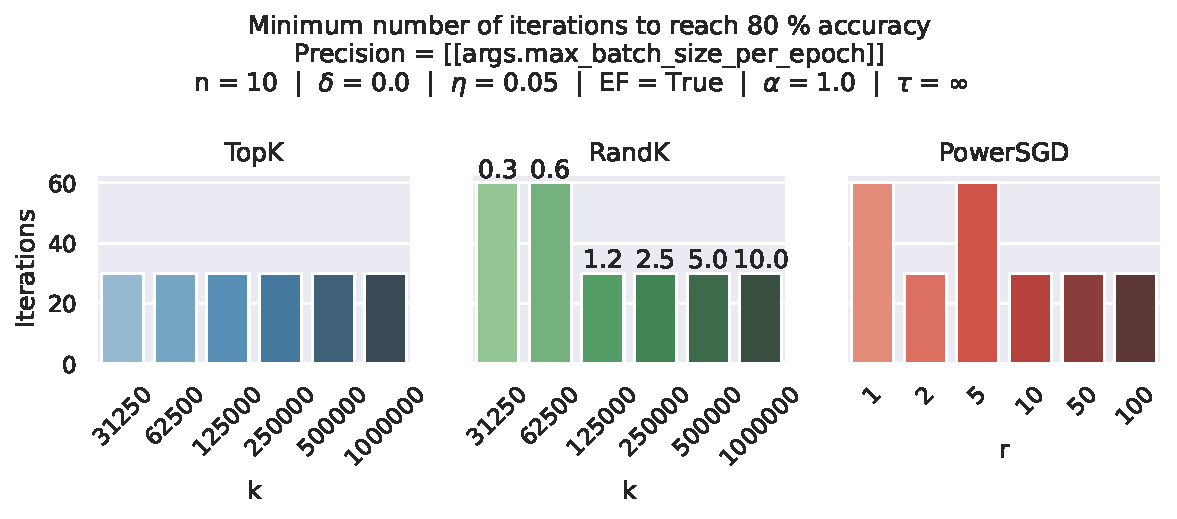
\includegraphics[scale=0.65]{figures/EXP_Compressors_Bars}
\caption{Comparison of various compressors. The $y$-axis has a logarithmic scale. The total throughput value is also reported on top of each bar (in MB).}\label{fig:compressors-bar}
\end{figure}


On Figure~\ref{fig:compressors-bar-bytes-per-iter} we see that for all three compressors, increasing the number of bytes sent at each iteration by using a larger $k$ or $r$ is not a good strategy for more efficient training as it increases linearly (slope $\approx$ 1) the total throughput needed to reach the desired accuracy. Hence it is better to use a large compression ratio (small $k$ and $r$).

\begin{figure}[h]
\centering
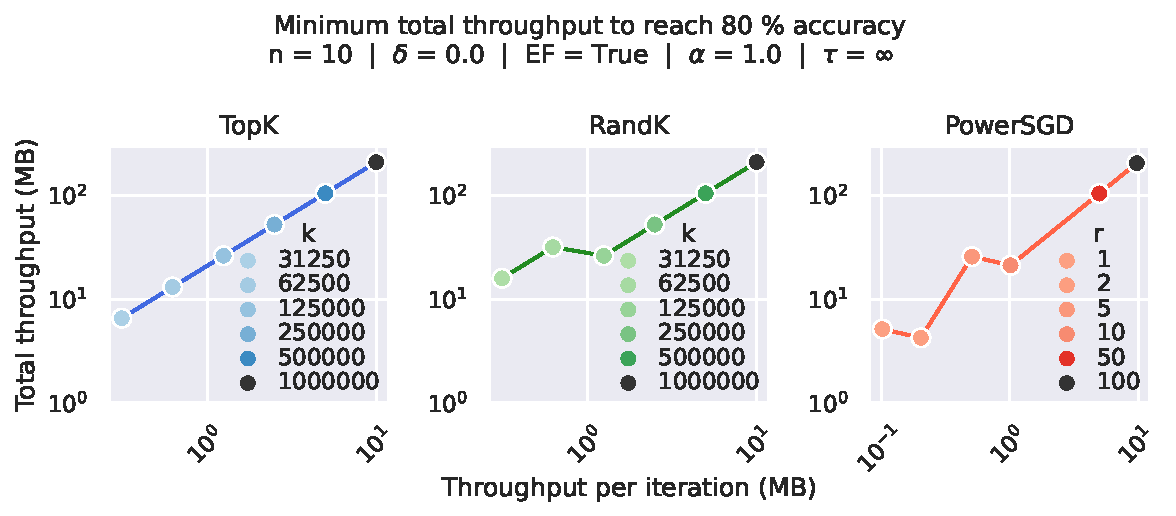
\includegraphics[scale=0.65]{figures/EXP_Compressors_Bars_By_Iter}
\caption{Relationship between the throughput per iteration and the total throughput to reach 80\% accuracy. Both axis have a logarithmic scale.}\label{fig:compressors-bar-bytes-per-iter}
\end{figure}


\paragraph{Byzantine workers}


On Figure~\ref{fig:clipping-zero} we observe that for all three attacks, the best learning curves are achieved by a small clipping radius ($\tau = 1$ for BF and IPM and $\tau=0.1$ for LoudBF).  When the clipping radius is too large ($\tau=10$) the attacks are more effective. For BF and IPM, when the clipping radius is very small ($\tau=0.1$) the learning curves are slowed down a bit compared to larger values of $\tau$, as it clips gradients from the good workers too much.

Interestingly, the momentum mechanism ($\alpha=0.1$, dotted line) usually makes convergence faster when there is no compression ($\hat\rho=1$, purple line) but slower when there is compression ($\hat\rho=0.25$, green line). We also see that when there is compression the attacks are more effective.

\begin{figure}[h]
\centering
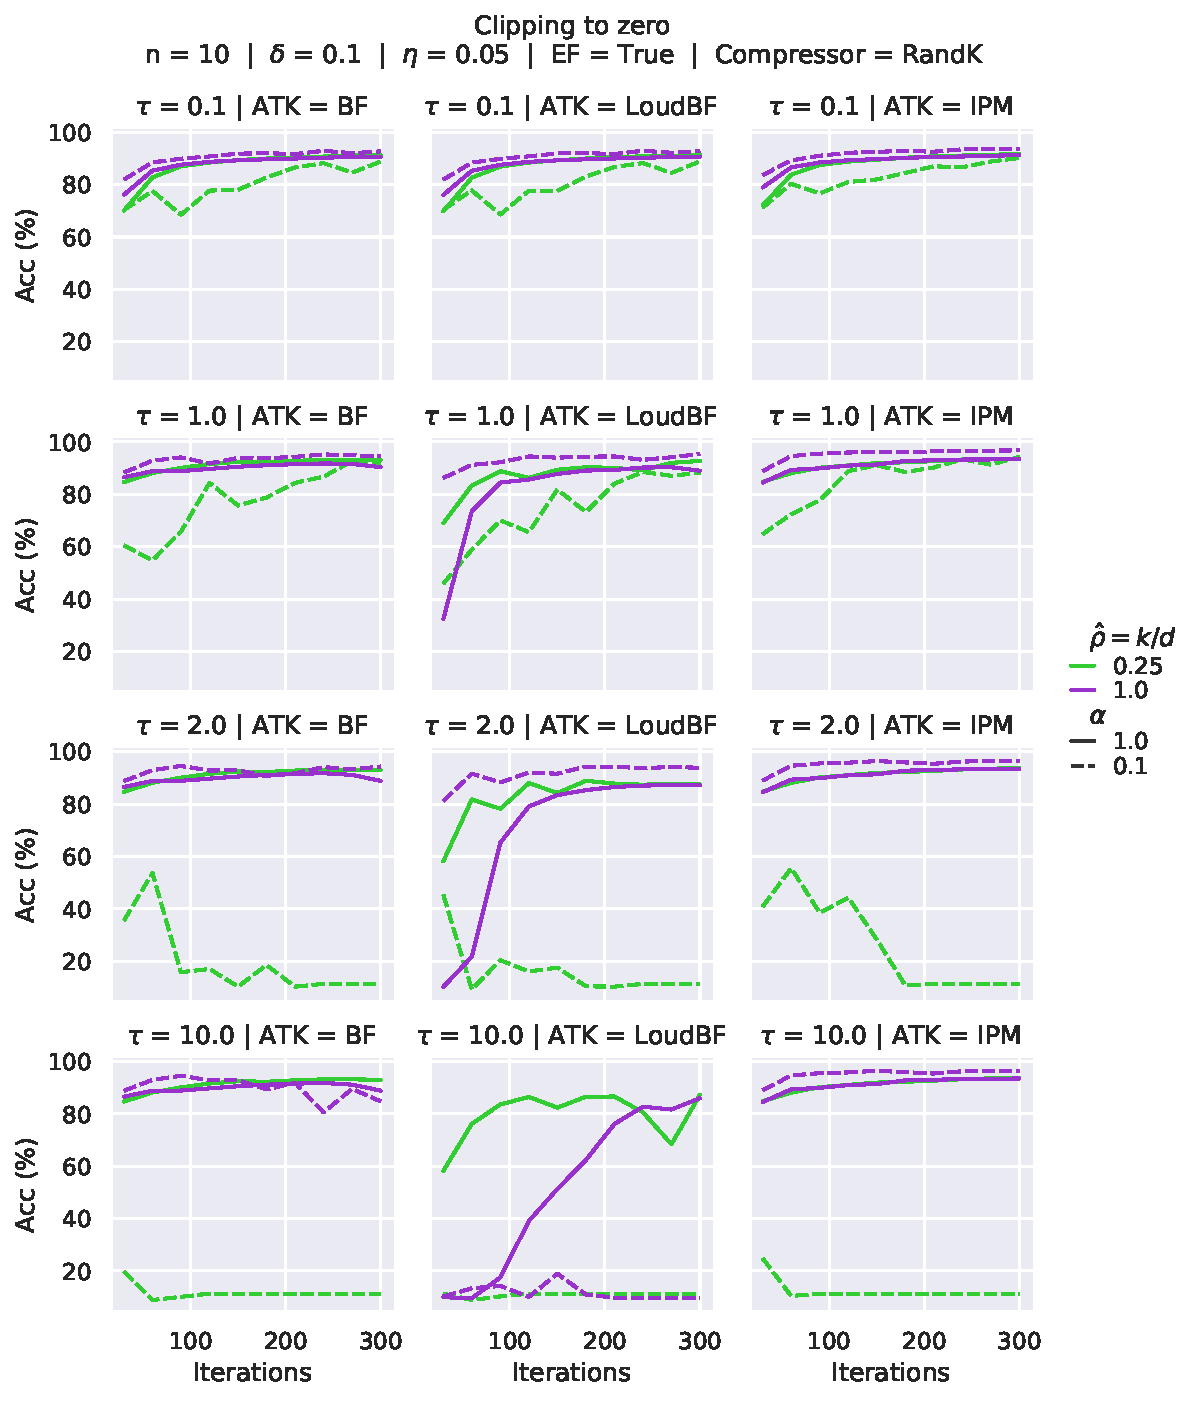
\includegraphics[scale=0.63]{figures/EXP_Clipping_Zero}
\caption{Learning curve for different attacks, momentum, clipping and compression parameters (clipping to zero)}\label{fig:clipping-zero}
\end{figure}

Centered clipping gives worse learning curves in general (see Figure~\ref{fig:clipping-centered} in Appendix~\ref{app:additional-plots}).



\section{Conclusion and future work}


In the context of federated learning with malicious workers we studied the performance of the standard distributed SGD algorithm improved with various mechanisms for robustness (momentum, clipping) and communication cost (compression with error feedback), keeping in mind they need to be compatible with a privacy-preserving implementation. We made a theoretical analysis of the convergence speed and empirical tests to investigate the gain of various compressors (Top-$k$, Random-$k$, PowerSGD) for the communication costs and the effectiveness of the defence mechanisms. Our tests suggest that, among our comparisons, PowerSGD is the most efficient compressor and the best defence mechanism is clipping to zero.

In the future, it would be interesting to study empirically the case where the good workers have non-iid data, which is more realistic. Also, the algorithm we discussed might be made more robust (with no privacy drawback) by incorporating a momentum mechanism on the server's side: the model update at step $t$ would be $\xx^{t+1} = \xx^t - \qq^{t+1}$, where 
\[
  \qq^{t+1} = (1-\beta) \qq^t + \beta \tfrac{1}{n} \tsum_{i=1}^n \cc_i^{t+1}
\]
for some $\beta$ in $(0,1]$, and starting with $\qq^1 = 0$.


\section*{Acknowledgements}

I am very grateful to Lie He for his supervision and very helpful support during this project, and to Prof.~Martin Jaggi and the MLO lab for hosting me and providing infrastructure and feedback for my work.


\printbibliography


\clearpage

\appendix


\section{Additional plots}\label{app:additional-plots}


On Figure~\ref{fig:clipping-centered} we make the same experiment as on Figure~\ref{fig:clipping-zero} but with centered clipping instead of clipping to zero. While for $\tau = 0.1, 1$ the clipping to zero strategy made the algorithm converge to high accuracy, this is not the case for centered clipping when momentum (dotted line) and compression (green line) are activated. In the case $\tau=0.1$ with momentum, even when there is no compression the learning process fails. This suggest favouring the clipping to zero strategy over centered clipping.

\begin{figure}[h]
\centering
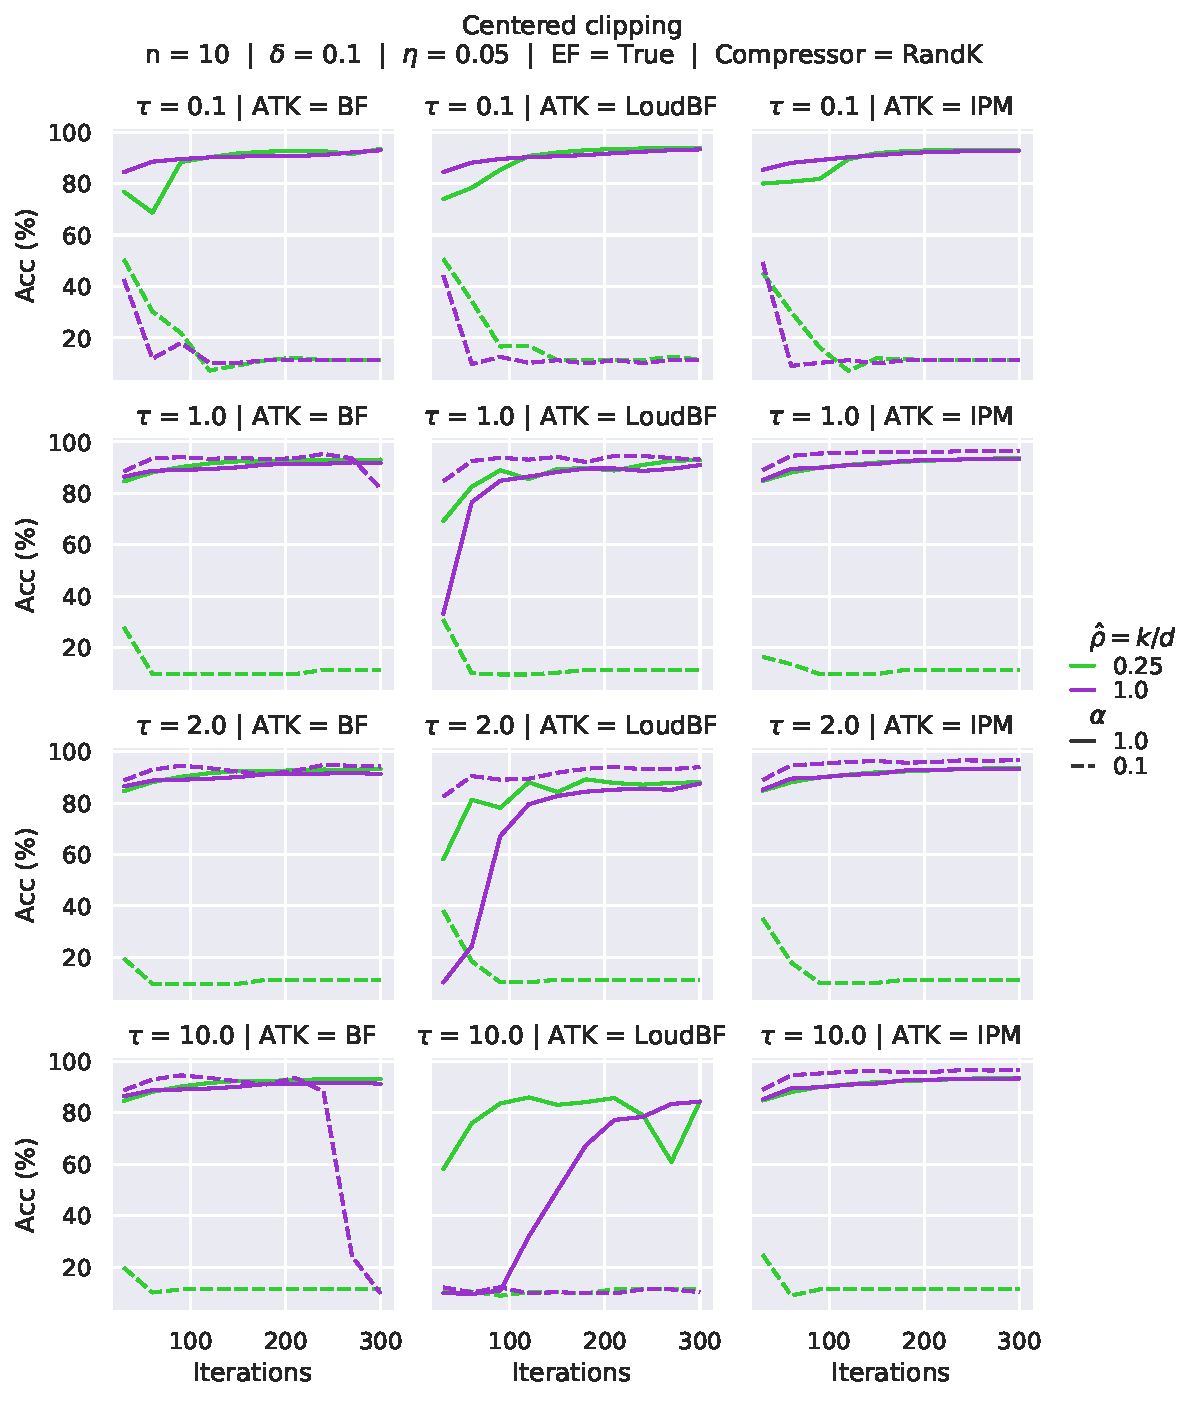
\includegraphics[scale=0.63]{figures/EXP_Clipping_Centered}
\caption{Learning curve for different attacks, momentum, clipping and compression parameters (centered clipping)}\label{fig:clipping-centered}
\end{figure}


\section{Technical lemmas}\label{app:technical-lemmas}

For simplicity we denote by $\E_t$ the conditional expectation  after realization of all the random variables $\xi_i$ up to and including step $t-1$ of the algorithm.

\begin{lemma}\label{lem:cosine-thm}
  For all vectors $\uu$ and $\vv$ we have
  \[
  2 \inp{\uu}{\vv} = \norm{\uu}^2 + \norm{\vv}^2 - \norm{\uu-\vv}^2 \, .
  \]
\end{lemma}

\begin{lemma}[Young's inequality, generalized]\label{lem:ineq-young-norm}
  Let $\uu$ and $\vv$ be vectors in an inner product space and let $\alpha > 0$. Then
  \[
    \norm{\uu + \vv}^2 \leq (1 + \alpha) \norm{\uu}^2 + (1 + 1/\alpha) \norm{\vv}^2 \, .
  \]
\end{lemma}

\begin{proof}
  Applying the Cauchy--Schwarz inequality and then the Young inequality we get
  \[
    \inp{\uu}{\vv}
    =
    \inp*{\sqrt \alpha \uu }{\vv / \sqrt \alpha}
    \leq
    \norm*{\sqrt \alpha \uu} \norm*{\vv / \sqrt \alpha}
    \leq
    \tfrac{1}{2} \norm*{\sqrt \alpha \uu}^2 + \tfrac{1}{2} \norm*{\vv / \sqrt \alpha}^2
    =
    \tfrac{\alpha}{2} \norm{\uu} + \tfrac{1}{2 \alpha} \norm{\vv}
  \]
  and then expanding the inner product we get
  \begin{align*}
    \norm{\uu+\vv}^2
     & =
    \norm{\uu}^2 + \norm{\vv}^2 + 2 \inp{\uu}{\vv}
    \leq
    \norm{\uu}^2 + \norm{\vv}^2 + \alpha \norm{\uu} + \tfrac{1}{\alpha} \norm{\vv}
    \\
     & =
    (1 + \alpha) \norm{\uu}^2 + (1 + 1/\alpha) \norm{\vv}^2
    \, .
  \end{align*}
\end{proof}


\begin{lemma}\label{lem:bound-by-avg-method}
  For every sequence $A_t$ satisfying 
  \begin{enumerate}
    \item $A_{t+1} \le (1-a) A_t + B_t$ for all $t \geq 1$,
    \item $A_1 \le C$,
  \end{enumerate}
  assuming $0 < a \le 1$ and $A_{T} \ge 0$, we have
  \[
    \tfrac{1}{T} \tsum_{t=0}^{T-1} A_{t+1}
     \le 
    \tfrac{C}{a T} + \tfrac{1}{a T} \tsum_{t=1}^{T-1} B_t \, .
  \]
\end{lemma}

\begin{proof}
  We have
  \begin{align*}
    \tsum_{t=0}^{T-1} A_{t+1}
     &=
    A_1 + \tsum_{t=1}^{T-1} A_{t+1}
     \le 
    C + \tsum_{t=1}^{T-1} ((1-a) A_t + B_t)
    \\     
     &=
    C + \tsum_{t=0}^{T-2} ((1-a) A_{t+1} + B_{t+1})
     =
    C + (1-a) \tsum_{t=0}^{T-2} A_{t+1}  + \tsum_{t=0}^{T-2} B_{t+1}
    \\
     & \le 
        C + (1-a) \tsum_{t=0}^{T-1} A_{t+1}  + \tsum_{t=1}^{T-1} B_t
  \end{align*}
  and regrouping the sums with $A_{t+1}$ on the left hand side we get 
  \[
    a \tsum_{t=0}^{T-1} A_{t+1}
     \le 
     C  + \tsum_{t=1}^{T-1} B_t \, .
  \]
  The result follows by dividing by $a T$.
\end{proof}


\begin{lemma}\label{lem:mean-norm-bound}
For all vectors $\aa_i$ we have 
\[
  \norm{\tfrac{1}{n} \tsum_{i=1}^n \aa_i}^2
   \le
  \tfrac{1}{n} \tsum_{i=1}^n \norm{\aa_i}^2
\]
\end{lemma}

\begin{proof}
We have   
  \begin{align*}
    \norm*{ \tfrac{1}{n} \tsum_{i=1}^n \aa_i }
    \leq
    \tsum_{i=1}^n \norm{\tfrac{1}{n} \aa_i}
    =
    \inp*{
      \begin{pmatrix} 1/n \\ \vdots \\ 1/n \end{pmatrix}
    }{
      \begin{pmatrix} \norm{\aa_1} \\ \vdots \\ \norm{\aa_n} \end{pmatrix}
    }
    \leq
    \tfrac{1}{\sqrt n} \sqrt{\tsum_{i=1}^n \norm{\aa_i}^2}
  \end{align*}
  where the first inequality comes from the triangle inequality and the second one is Cauchy--Schwarz.
\end{proof}


\begin{lemma}\label{lem:mean-norm-bound-indep}
If $\aa_i$ are zero mean independent random variables with $\E \norm{\aa_i}^2 \leq A$ for all $i$ then we have $\E \inp{\aa_i}{\aa_j} = 0$ for all $i \neq j$ hence
\[
  \E \norm{\tfrac{1}{n} \tsum_{i=1}^n \aa_i}^2
   \le
  \tfrac{A}{n}
\]
\end{lemma}


\begin{lemma}\label{lem:gradient-bounds}
  We have
  \[
    \E_t \tfrac{1}{n} \tsum_{i=1}^n \gg_i^t = \nabla f(\xx^t)
  \]
  and
  \[
    \tfrac{1}{n} \tsum_{i=1}^n \E_t \norm{\gg_i^t - \nabla f(\xx^t)}^2 \le \sigma^2 + \zeta^2 \, .
  \]
\end{lemma}

\begin{proof}
  Interchanging derivatives and expectation we get
  \[
    \E_t \gg_i^{t+1} 
    = \E_t \nabla f_i(\xx^t; \xi_i^t)
    = \nabla \E_t f_i(\xx^t; \xi_i^t)
  \]
  hence
  \[
    \E_t \tfrac{1}{n} \tsum_{i=1}^n \gg_i^{t+1}
    =
    \nabla \tfrac{1}{n} \tsum_{i=1}^n \E_t f_i(\xx^t; \xi_i^t)
    =
    \nabla f(\xx^t)    
  \]
  as $f = \tfrac{1}{n} \tsum_{i=1}^n f_i$.
  
  For the second part, for every $t$ we have
  \begin{align*}
    \E_t \norm{\gg_i^{t+1} - \nabla f(\xx^t)}^2
     & =
    \E_t \norm{\gg_i^{t+1} - \E_t \gg_i^{t+1}}^2
    + \norm{\E_t \gg_i^{t+1} - \nabla f(\xx^t)}^2
  \end{align*}
  because the inner product $\inp{\gg_i^{t+1} - \E_t \gg_i^{t+1}}{\E_t \gg_i^{t+1} - \nabla f(\xx^t)}$ has expectation.zero. Taking the average over $i$ yields
  \[
    \tfrac{1}{n} \tsum_{i=1}^n \E_t \norm{\gg_i^{t+1} - \nabla f(\xx^t)}^2 
     \le 
    \sigma^2 + \zeta^2
  \]
  thanks to the noise bound (Assumption~\ref{assum:noise-bound}) and to the heterogeneity bound (Assumption~\ref{assum:heterogeneity-bound}), and using $\gg_i^{t+1} = \nabla f_i(\xx^t; \xi_i^t)$.

\end{proof}



\section{Proofs}\label{app:proofs}


\subsection{No malicious workers}


\begin{theorem}[Lemma~\ref{lem:efsgd-convergence} in Section~\ref{sec:theoretical-results}]\label{app:thm:efsgd-convergence}
If the step-size $\eta$ is at most $\tfrac{\rho}{\sqrt{24} L}$ then for Algorithm~\ref{algo:fedsgd} without momentum ($\alpha=1$) and without clipping we have
  \[
    \tfrac{1}{T} \tsum_{t=0}^{t-1} \E \norm{\nabla f(\xx^t)}^2
    \leq
    \tfrac{8}{\eta T}(f(\xx^0) - f^\ast) + \eta L (\sigma^2+\zeta^2) \bigl(\sqrt{24} (1/\rho-1) + 4/n\bigr)
  \]
\end{theorem}

\begin{proof}
  For simplicity we use shorthand notations for the averages $\gg^{t+1} := \tfrac{1}{n} \tsum_{i=1}^n \gg_i^{t+1}$ and $\bm r^{t+1} := \tfrac{1}{n} \tsum_{i=1}^n \bm r_i^{t+1}$ and also $\pp_i^{t+1} := \eta \gg_i^{t+1} + \bm r_i^t$.
  
  Let us study the sequence $\tilde \xx^t := \xx^t - \bm r^t$. Observe that
  \begin{align*}
    \tilde \xx^{t+1}
     & =
    \xx^{t+1} - \bm r^{t+1}
    =
    \xx^t - \tfrac{1}{n} \tsum_{i=1}^n \mathcal C(\pp_i^{t+1}) - \tfrac{1}{n} \tsum_{i=1}^n (\pp_i^{t+1} - \mathcal C(\pp_i^{t+1}))
    =
    \xx^t - \tfrac{1}{n} \tsum_{i=1}^n \pp_i^{t+1}
    \\
     & =
    \xx^t -  \tfrac{1}{n} \tsum_{i=1}^n \eta \gg_i^{t+1} - \tfrac{1}{n} \tsum_{i=1}^n \bm r_i^t
    =
    \xx^t - \eta \gg^{t+1} - \bm r^t
    =
    \tilde \xx^t - \eta \gg^{t+1}
  \end{align*}
  hence $\tilde \xx^{t+1} - \tilde \xx^t = -\eta \gg^{t+1}$. 

  Later in the proof we will need an upper bound on the average distance (over $t$) between $\nabla f(\tilde \xx^t)$ and $\nabla f(\xx^t)$, so let us compute it. For every $t$ we have
  \[
    \norm*{\nabla f(\tilde \xx^t) - \nabla f(\xx^t)}^2
    \leq
    L^2 \norm{\tilde \xx^t - \xx^t}^2
    =
    L^2 \norm{\bm r^t}^2
    \le
    \tfrac{L^2}{n} \tsum_{i=1}^n \norm{\bm r_i^t}^2
  \]
  where for the last inequality we used Lemma~\ref{lem:mean-norm-bound}.
  Let us upper bound the squared norm of each $\bm r_i^t$ for all $i$. We have
  \begin{align*}
    \norm{\bm r_i^t}^2
     & =
    \norm{\pp_i^t - \mathcal C(\pp_i^t)}^2
    \leq
    (1-\rho) \norm{\pp_i^t}^2
    \\
     & \leq
    (1-\rho) (1 + 2/\rho) \eta^2 \norm{\gg_i^t}^2 + (1-\rho)  (1 + \rho/2) \norm{\bm r_i^{t-1}}^2
  \end{align*}
  where for the last inequality we applied Lemma~\ref{lem:ineq-young-norm} with the constant $\alpha := \rho/2$. Since $(1-\rho)(1+2/\rho) \leq (1-\rho) (1/\rho+2/\rho) = 3(1-\rho)/\rho$ (because $0 < \rho \leq 1$) and $(1-\rho)(1+\rho/2) = 1 - \rho/2 - \rho^2/2 < 1 - \rho/2$ we obtain the simplified upper bound
  \[
    \norm{\bm r_i^t}^2
    \leq
    \tfrac{3 \eta^2 (1-\rho)}{\rho} \norm{\gg_i^t}^2 + (1-\rho/2) \norm{\bm r_i^{t-1}}^2
    \, .
  \]
  Summing over $t$ yields
  \begin{align*}
    \tsum_{t=0}^{T-1} \norm{\bm r_i^t}^2
     & =
    \tsum_{t=1}^{T-1} \norm{\bm r_i^t}^2
    \leq
    \tfrac{3 \eta^2 (1-\rho)}{\rho} \tsum_{t=1}^{T-1}  \norm{\gg_i^t}^2 + (1-\rho/2) \tsum_{t=1}^{T-1}  \norm{\bm r_i^{t-1}}^2
    \\
     & =
    \tfrac{3 \eta^2 (1-\rho)}{\rho} \tsum_{t=0}^{T-2}  \norm{\gg_i^{t+1}}^2 + (1-\rho/2) \tsum_{t=0}^{T-2}  \norm{\bm r_i^t}^2
    \\
     & \leq
    \tfrac{3 \eta^2 (1-\rho)}{\rho} \tsum_{t=0}^{T-1}  \norm{\gg_i^{t+1}}^2 + (1-\rho/2) \tsum_{t=0}^{T-1}  \norm{\bm r_i^t}^2
  \end{align*}
  where the first equality is because $\bm r_i^0 = 0$ in each client $i$, the second equality is a change of indices and the last inequality is an upper bound by taking an additional term with index $t = T-1$ in the sums. Putting the sum with the norm of the $\bm r_i^t$ on the left hand side we get
  \[
    \tsum_{t=0}^{T-1} \norm{\bm r_i^t}^2
    \leq
    \tfrac{6 \eta^2 (1-\rho)}{\rho^2} \tsum_{t=0}^{T-1}  \norm{\gg_i^{t+1}}^2
  \]
  Combining this with the previous upper bound on the distance between $\nabla f(\tilde \xx^t)$ and $\nabla f(\xx^t)$ we obtain the following upper bound:
  \[
    \tsum_{t=0}^{T-1} \norm{\nabla f(\tilde \xx^t) - \nabla f(\xx^t)}^2
    \leq
    \tfrac{6 \eta^2 L^2 (1-\rho)}{n \rho^2} \tsum_{t=0}^{T-1} \tsum_{i=1}^n \norm{\gg_i^{t+1}}^2
    \, .
  \]
  Moreover for every $t$ we have
  \begin{align*}
    \tsum_{i=1}^n \E_t \norm{\gg_i^{t+1}}^2
     & =
    \tsum_{i=1}^n \E_t \norm{\gg_i^{t+1} - \nabla f(\xx^t) + \nabla f(\xx^t)}^2 
    \\
     & =
    \tsum_{i=1}^n \left( \E_t \norm{\gg_i^{t+1} - \nabla f(\xx^t)}^2  + \norm{\nabla f(\xx^t)}^2 + \E_t \inp*{\gg_i^{t+1} - \nabla f(\xx^t)}{\nabla f(\xx^t)} \right)
    \\
     & \leq
    n (\sigma^2+\zeta^2) + n \norm{\nabla f(\xx^t)}^2 + n \inp*{\E_t [\gg^t]  - \nabla f(\xx^t)}{\nabla f(\xx^t)}
    \\
     & =
    n (\sigma^2+\zeta^2) + n \norm{\nabla f(\xx^t)}^2
  \end{align*}
  using Lemma~\ref{lem:gradient-bounds} for the inequality.
  Hence we obtain (taking unconditional expectation) the following upper bound that we will use later on:
  \[
    \tsum_{t=0}^{T-1} \E \norm{\nabla f(\tilde \xx^t) - \nabla f(\xx^t)}^2
    \leq
    \tfrac{6 \eta^2 L^2 (1-\rho)}{\rho^2} \bigl( T (\sigma^2+\zeta^2) + \tsum_{t=0}^{T-1} \E \norm{\nabla f(\xx^t)}^2 \bigr)
    \, .
  \]
  For every $t$, using the Lipschitz condition on $\nabla f$ we get
  \begin{align*}
    f(\tilde \xx^{t+1})
     & \leq
    f(\tilde \xx^t) + \inp{\nabla f(\tilde \xx^t)}{\tilde \xx^{t+1} - \tilde \xx^t} + \tfrac{L}{2} \norm{\tilde \xx^{t+1} - \tilde \xx^t}^2
    \\
     & =
    f(\tilde \xx^t) + \inp{\nabla f(\tilde \xx^t)}{-\eta \gg^{t+1}} + \tfrac{L \eta^2}{2} \norm{\gg^{t+1}}^2
    \, .
  \end{align*}
  Taking conditional expectation on both sides yields
  \begin{align*}
    \E_t f(\tilde \xx^{t+1}) 
     & \leq
    f(\tilde \xx^t) + \inp{\nabla f(\tilde \xx^t)}{-\eta \nabla f(\xx^t)} + \tfrac{L \eta^2}{2} \E_t \norm{\gg^{t+1}}^2
    \\
     & \leq
    f(\tilde \xx^t) + \inp*{\nabla f(\tilde \xx^t)}{-\eta \nabla f(\xx^t)} + \tfrac{L \eta^2}{2} \left( \norm{\nabla f(\xx^t)}^2  + (\sigma^2+\zeta^2)/n\right)
    \, .
  \end{align*}
  Now we upper bound the middle term:
  \begin{align*}
    \inp{\nabla f(\tilde \xx^t)}{-\eta \nabla f(\xx^t)}
     & =
    \inp{\nabla f(\xx^t)}{-\eta \nabla f(\xx^t)} +   \inp{\nabla f(\tilde \xx^t) - \nabla f(\xx^t)}{-\eta \nabla f(\xx^t)}
    \\
     & \leq
    -\eta \norm{\nabla f(\xx^t)}^2 + \eta \norm{\nabla f(\tilde \xx^t) - \nabla f(\xx^t)} \norm{\nabla f(\xx^t)}
    \\
     & \leq
    -\eta \norm{\nabla f(\xx^t)}^2 + \eta \left( \tfrac{1}{2} \norm{\nabla f(\tilde \xx^t) - \nabla f(\xx^t)}^2 + \tfrac{1}{2} \norm{\nabla f(\xx^t)}^2 \right)
    \\
     & =
    -\tfrac{\eta}{2} \norm{\nabla f(\xx^t)}^2 + \tfrac{\eta}{2} \norm{\nabla f(\tilde \xx^t) - \nabla f(\xx^t)}^2
  \end{align*}
  where for the first inequality we used the Cauchy--Schwarz inequality and for the second inequality we used Young's inequality. Combining with the previous computation we get
  \begin{align*}
    \E_t f(\tilde \xx^{t+1})  - f(\tilde \xx^t)
     & \leq
    -\tfrac{\eta}{2} \norm{\nabla f(\xx^t)}^2 + \tfrac{\eta}{2} \norm{\nabla f(\tilde \xx^t) - \nabla f(\xx^t)}^2 + \tfrac{L \eta^2}{2} \left( \norm{\nabla f(\xx^t)}^2  + (\sigma^2+\zeta^2)/n\right)
    \\
     & =
    \tfrac{L\eta^2-\eta}{2} \norm{\nabla f(\xx^t)}^2 + \tfrac{\eta}{2} \norm{\nabla f(\tilde \xx^t) - \nabla f(\xx^t)}^2 + \tfrac{L \eta^2 (\sigma^2+\zeta^2)}{2n}
  \end{align*}
  Now we take the sum over $t$ on both sides
  \begin{align*}
    \tsum_{t=0}^{T-1} \left( \E_t f(\tilde \xx^{t+1}) - f(\tilde \xx^t) \right)
     & \leq
    \tfrac{L\eta^2-\eta}{2} \tsum_{t=0}^{T-1} \norm{\nabla f(\xx^t)}^2 
    \\
     & \quad 
    + \tfrac{\eta}{2} \tsum_{t=0}^{T-1} \norm{\nabla f(\tilde \xx^t) - \nabla f(\xx^t)}^2 + \tfrac{T L \eta^2 (\sigma^2+\zeta^2)}{2n} \, .
  \end{align*}
  Taking unconditional expectation on both sides we get
  \begin{align*}
    \tsum_{t=0}^{T-1} \left(\E f(\tilde \xx^{t+1}) - \E f(\tilde \xx^t)\right)
     & \leq
    \tfrac{L\eta^2-\eta}{2} \tsum_{t=0}^{T-1} \E \norm{\nabla f(\xx^t)}^2
    \\
     & \quad
    + \tfrac{\eta}{2} \E \tsum_{t=0}^{T-1} \norm{\nabla f(\tilde \xx^t) - \nabla f(\xx^t)}^2 
    + \tfrac{T L \eta^2 (\sigma^2+\zeta^2)}{2n}
    \, .
  \end{align*}
  We notice that the left hand side is a telescoping sum. On the right hand side we use the upper bound we computed at the beginning for the middle term:
  \begin{align*}
    \E f(\tilde \xx^T) - f(\xx^0)
     & \leq
    \tfrac{L\eta^2-\eta}{2} \tsum_{t=0}^{T-1} \E \norm{\nabla f(\xx^t)}^2
    \\
     & \quad
    + \tfrac{3 \eta^3 L^2 (1-\rho)}{\rho^2} \bigl( T (\sigma^2+\zeta^2) + \tsum_{t=0}^{T-1} \E \norm{\nabla f(\xx^t)}^2 \bigr)
    + \tfrac{T L \eta^2 (\sigma^2+\zeta^2)}{2n}
  \end{align*}
  and rearranging we obtain
  \[
    \left(-\tfrac{L\eta^2-\eta}{2} - \tfrac{3\eta^3 L^2 (1-\rho)}{\rho^2}\right) \tsum_{t=0}^{T-1} \E \norm{\nabla f(\xx^t)}^2
    \leq
    (f(\xx^0) - f^\ast) + \tfrac{3 T L^2 \eta^3 (\sigma^2+\zeta^2) (1-\rho)}{\rho^2} + \tfrac{TL \eta^2 (\sigma^2+\zeta^2)}{2n}
  \]
  since $\expec{f(\tilde \xx^T)} \ge f^\ast$. Let us simplify a bit the expressions on the left hand side. We have $\eta \leq \rho / (\sqrt{24}L)$ so
  \[
    \tfrac{3\eta^3 L^2 (1-\rho)}{\rho^2} 
     \le 
    \tfrac{3\eta (1-\rho)}{24} 
     = 
    \tfrac{\eta (1-\rho)}{8} 
     \le 
    \tfrac{\eta}{8}
  \]
  and also $\eta \le 1/(2L)$ (as a looser bound) so
  \[
    \tfrac{L\eta^2 - \eta}{2} 
     \le 
    \tfrac{\eta/2 - \eta}{2} = -\eta / 4 \, .
  \]
  Combining these two gives
  \[
    -\tfrac{L\eta^2-\eta}{2} - \tfrac{3\eta^3 L^2 (1-\rho)}{\rho^2} 
     \ge 
    -\tfrac{\eta}{8} +\tfrac{\eta}{4} 
     = 
    \tfrac{\eta}{8}
  \]
  so we obtain
  \[
    \tsum_{t=0}^{T-1} \E \norm{\nabla f(\xx^t)}^2 
    \leq
    \tfrac{8(f(\xx^0) - f^\ast)}{\eta} + \tfrac{24 T L^2 \eta^2 (\sigma^2+\zeta^2) (1-\rho)}{\rho^2} + \tfrac{4 TL \eta (\sigma^2+\zeta^2)}{n}
  \]
  and then the statement of the lemma by dividing by $T$ and using $\eta \leq \rho/ (\sqrt{24} L)$.
\end{proof}


Let us analyse the convergence rate implied by our bound from Lemma~\ref{lem:efsgd-convergence}. The upper bound is of the form $G(\eta) = A/\eta + B \eta$ with
\[
  A = \tfrac{8(f(\xx^0) - f^\ast)}{T}
\]
and
\[
  B = \tfrac{\sqrt{24} L (\sigma^2+\zeta^2) (1-\rho)}{\rho} + \tfrac{4 L (\sigma^2+\zeta^2)}{n}
\]
so it is minimized for the step-size $\eta^\ast = \sqrt{A/B}$ for which it becomes
\[
  G(\eta^\ast)
  =
  2\sqrt{AB}
  =
  2 \left(\tfrac{8(f(\xx_0) - f^\ast)}{T} \right)^{1/2} \left(\tfrac{\sqrt{24} L (\sigma^2+\zeta^2) (1-\rho)}{\rho} + \tfrac{4 L (\sigma^2+\zeta^2)}{n}\right)^{1/2} \, .
\]
This gives the corollary below.


\begin{corollary}[Convergence rate of the EF-SGD, Corollary~\ref{cor:efsgd-convergence-rate} in Section~\ref{sec:theoretical-results}]\label{app:cor:efsgd-convergence-rate}
  With step size 
  \[
  	\eta = \left(8(f(\xx^0) - f^\ast)\right)^{1/2} \left(T  (\sigma^2+\zeta^2) \bigl(\sqrt{24} (1/\rho - 1) + 4 / n\bigr)\right)^{-1/2}
  \]
  and number of iterations 
  \[
    T \geq \tfrac{32 L}{\varepsilon^2} (\sigma^2+\zeta^2) (f(\xx^0) - f^\ast) \Bigl(\tfrac{4}{n} + \sqrt{24} \bigl(\tfrac{1}{\rho} - 1\bigr)\Bigr)
  \]
  we have
  \[
    \tfrac{1}{T} \tsum_{t=0}^{T-1} \E \norm{\nabla f(\xx^t)}^2 \leq \varepsilon
  \]
  so $T = O(\varepsilon^2)$. If $\rho = 1$ (no compression) we recover linear scalability in the number of workers $n$, i.e. $T = O(1/n)$. The compression parameter $\rho$ slows down the convergence linearly, i.e. $T = O(1/\rho)$.
\end{corollary}


\subsection{Byzantine workers}


For simplicity we use the notation $\uu_{\gset'} = \tfrac{1}{|\gset'|} \tsum_{i\in\gset'} \uu_i$ for any subset of good workers $\gset' \subseteq \gset$.

\begin{theorem}[Lemma~\ref{lem:convergence-byz} in Section~\ref{sec:theoretical-results}]\label{app:thm:convergence-byz}
  If $\eta \le \tfrac{1}{2L}$ then
  \begin{align*}
    & \left(1 - 2 \delta - \tfrac{144(1-\delta)(1-\rho)}{\rho^2} \right) \tfrac{1}{T} \tsum_{t=0}^{T-1} \E \norm{\nabla f(\xx^t)}^2 
    \\
     & \qquad + 
    \left( \tfrac{1}{2} - \tfrac{18(1-\delta)(1-\alpha)^2 L^2 \eta^2}{\alpha^2} \right) \tfrac{1}{T} \tsum_{t=0}^{T-1} \E \norm{\tfrac{1}{n \eta}\tsum_{i=1}^n \cc_i^{t+1}}^2
    \\
     & \le  
    \tfrac{2(f(\xx^0) - f^\ast)}{\eta T}
     + 
    \tfrac{2\delta\tau^2}{\eta^2}
     + 
    \tfrac{2}{n \eta^2 T} \tsum_{t=0}^{T-1} \tsum_{i\in\gfset} (\E \norm{ \vv_i^{t+1} } - \tau)^2 
    \\
     & \qquad + 
    \tfrac{72(1-\delta)(1-\rho)}{\rho^2} 
      \left(      
          2  \zeta^2
        + \alpha\sigma^2                                             
        + \tfrac{1}{\alpha T}(2\norm{\nabla f(\xx^0) }^2
        + 2 \zeta^2
        + \sigma^2)
      \right)
     +
    \tfrac{6\sigma^2}{n} \left(\alpha + \tfrac{1}{\alpha T}\right) \, .
  \end{align*}
\end{theorem}

\begin{proof}
  Use Lemma~\ref{lem:suff-decrease}, the error decomposition from Lemma~\ref{lem:error-decomposition} and bound the error from the bad workers with Lemma~\ref{lem:error-bad-workers} and the error from the good workers by Lemma~\ref{lem:error-good-workers}. 
  \begin{align*}
    &\tfrac{1}{T} \tsum_{t=0}^{T-1} \E \norm{\nabla f(\xx^t)}^2 
     + 
    \tfrac{1}{2T} \tsum_{t=0}^{T-1} \E \norm{\tfrac{1}{n \eta}\tsum_{i=1}^n \cc_i^{t+1}}^2
     \le
    \tfrac{2(f(\xx^0) - f^\ast)}{\eta T} + \delta \E \cE_\bset + (1-\delta) \E \cE_\gset
    \\
     &\le  
    \tfrac{2(f(\xx^0) - f^\ast)}{\eta T}
    + 
    \delta \left(\tfrac{2\tau^2}{\eta^2} + \tfrac{2}{T} \tsum_{t=0}^{T-1} \E \norm{ \nabla f(\xx^t) }^2 \right)
    \\
     & \quad + 
    \tfrac{2(1-\delta)}{\eta^2 T |\gset|} \tsum_{t=0}^{T-1} \tsum_{i\in\gfset} (\E \norm{ \vv_i^{t+1} } - \tau)^2 
    \\
     & \quad + 
    \tfrac{72(1-\delta)(1-\rho)}{\rho^2} 
      \left(      
        \tfrac{2}{T}\tsum_{t=1}^{T-1} \E \norm{\nabla f(\xx^t) }^2
        +  2  \zeta^2
        + \alpha\sigma^2                                             
        + \tfrac{1}{\alpha T}(2\norm{\nabla f(\xx^0) }^2
        + 2 \zeta^2
        + \sigma^2)
      \right)
    \\
     & \quad +
    \tfrac{18(1-\delta)(1-\alpha)^2 L^2}{\alpha^2T} \tsum_{t=1}^{T-1}
    \norm{ \tfrac{1}{n} \tsum_{i=1}^n \cc_i^t }^2
    + (1-\delta) \left(\tfrac{6\alpha\sigma^2}{|\gset|} + \tfrac{6\sigma^2}{\alpha T|\gset|}\right)
  \end{align*}
  We obtain the result of the theorem by moving the terms with $\norm{\nabla f(\xx^t)}^2$ and $\norm{\cc_i^t}^2$ on the left hand side, and reindexing in the sum with $\norm{\cc_i^t}^2$.
\end{proof}


\begin{lemma}\label{lem:suff-decrease}
  If $\eta \le \tfrac{1}{2L}$ then
  \begin{align*}
    \tfrac{1}{T} \tsum_{t=0}^{T-1} \norm{\nabla f(\xx^t)}^2 
     + 
    \tfrac{1}{2T} \tsum_{t=0}^{T-1} \norm*{\tfrac{1}{n \eta}\tsum_{i=1}^n \cc_i^{t+1}}^2
     \leq 
    \tfrac{2(f(\xx^0) - f^\ast)}{\eta T} + \cE
  \end{align*}
  where 
  \begin{align*}
    \cE = \tfrac{1}{T} \tsum_{t=0}^{T-1} \underbrace{ \norm*{\tfrac{1}{n\eta} \tsum_{i=1}^n \cc_i^{t+1} - \nabla f(\xx^t)}^2}_{\cE^{t+1}} \, .
  \end{align*}
\end{lemma}

\begin{proof}
  Since $f$ is $L$-smooth we have
  \[
    f(\xx^{t+1}) \le f(\xx^t) + \inp{\nabla f(\xx^t)}{\xx^t - \xx^{t+1}} + \tfrac{L}{2} \norm{\xx^t - \xx^{t+1}}^2
  \]
  and then, using Lemma~\ref{lem:cosine-thm} and the fact that $\xx^{t+1} - \xx^t = \tfrac{1}{n} \tsum_{i=1}^n \cc_i^{t+1}$,
  \begin{align*}
    &\inp{\nabla f(\xx^t)}{\xx^t - \xx^{t+1}} + \tfrac{L}{2} \norm{\xx^t - \xx^{t+1}}^2 
    \\
    &=
    -\inp{\sqrt{\eta} \nabla f(\xx^t)}{\tfrac{1}{n\sqrt\eta} \tsum_{i=1}^n \cc_i^{t+1}} + \tfrac{L \eta^2}{2} \norm{\tfrac{1}{n\eta} \tsum_{i=1}^n \cc_i^{t+1}}^2
    \\
    &= -\tfrac{\eta}{2} \norm{\nabla f(\xx^t)} - \left( \tfrac{\eta}{2} - \tfrac{L\eta^2}{2}\right) \norm{\tfrac{1}{n\eta} \tsum_{i=1}^n \cc_i^{t+1}}^2 + \tfrac{\eta}{2} \norm{\tfrac{1}{n\eta} \tsum_{i=1}^n \cc_i^{t+1} - \nabla f(\xx^t)}^2
  \end{align*}
  hence
  \[
    \tfrac{\eta}{2} \norm{\nabla f(\xx^t)} 
    + \left( \tfrac{\eta}{2} - \tfrac{L\eta^2}{2}\right) \norm{\tfrac{1}{n\eta} \tsum_{i=1}^n \cc_i^{t+1}}^2 
    \le 
   f(\xx^t) - f(\xx^{t+1}) 
   + \tfrac{\eta}{2} \norm{\tfrac{1}{n\eta} \tsum_{i=1}^n \cc_i^{t+1} - \nabla f(\xx^t)}^2
  \]
  Since $\eta \le \tfrac{1}{2L}$ we have $\tfrac{\eta}{4} \le \tfrac{\eta}{2} - \tfrac{L\eta^2}{2}$ hence
  \[
    \tfrac{\eta}{2} \norm{\nabla f(\xx^t)} 
    + \tfrac{\eta}{4} \norm{\tfrac{1}{n\eta} \tsum_{i=1}^n \cc_i^{t+1}}^2 
    \le 
   f(\xx^t) - f(\xx^{t+1}) 
   + \tfrac{\eta}{2} \norm{\tfrac{1}{n\eta} \tsum_{i=1}^n \cc_i^{t+1} - \nabla f(\xx^t)}^2 \, .
  \]
  Taking the average over $t$ the term $f(\xx^t) - f(\xx^{t+1})$ becomes a telescoping sum, and the result follows by dividing the equation by $\tfrac{\eta}{2}$.
\end{proof}

  
\begin{lemma}[Error decomposition]\label{lem:error-decomposition}
  From the convexity of the Euclidean norm function $\norm{\cdot}^2$ we immediately get
  \begin{align*}
    \mathcal E
     \le 
    \tfrac{|\bset|}{n} \cE_\bset
     + 
    \tfrac{|\gset|}{n} \cE_\gset
  \end{align*}
  where 
  \[
    \cE_\bset = \tfrac{1}{T} \tsum_{t=0}^{T-1} \norm*{\tfrac{1}{\eta |\bset|} \tsum_{i\in\bset} \cc_i^{t+1} - \nabla f(\xx^t)}^2
  \]
  (error from the bad workers) and similarly for $\cE_\gset$ (error from the good workers).
\end{lemma}


\begin{lemma}[Error from the bad workers]\label{lem:error-bad-workers}
  \begin{align*}
    \tfrac{1}{T} \tsum_{t=0}^{T-1} \cE_\bset^{t+1} 
     \le 
    \tfrac{2\tau^2}{\eta^2} + \tfrac{2}{T} \tsum_{t=0}^{T-1} \norm{ \nabla f(\xx^t) }^2  
  \end{align*}
\end{lemma}

\begin{proof}
  Using Young's inequality
  \begin{align*}
    \cE_\bset^{t+1} 
     =
    \norm*{\tfrac{1}{\eta |\bset|} \tsum_{i\in\bset} \cc_i^{t+1} - \nabla f(\xx^t)}^2 
     \le 
    2\norm*{\tfrac{1}{\eta |\bset|} \tsum_{i\in\bset} \cc_i^{t+1}}^2 
    + 2 \norm{\nabla f(\xx^t)}^2  
  \end{align*}
  and by Lemma~\ref{lem:mean-norm-bound} 
  \[
    \norm*{\tfrac{1}{\eta |\bset|} \tsum_{i\in\bset} \cc_i^{t+1}}^2 
     \le 
    \tfrac{1}{\eta^2 |\bset|} \tsum_{i\in\bset} \norm{\cc_i^{t+1}}^2 
     \le 
    \tfrac{\tau^2}{\eta^2 |\bset|}
  \]
Combining these two bounds and taking the average over $t$ gives the result.
\end{proof}


\begin{lemma}[Error from the good workers]\label{lem:error-good-workers}
\begin{align*}
  \tfrac{1}{T} \tsum_{t=0}^{T-1} \E \cE_\gset^{t+1} 
   &\le
  \tfrac{2}{\eta^2 T |\gset|} \tsum_{t=0}^{T-1} \tsum_{i\in\gfset} (\E \norm{ \vv_i^{t+1} } - \tau)^2
  \\
   & \quad + 
  \tfrac{72(1-\rho)}{\rho^2} 
    \left(      
      \tfrac{2}{T}\tsum_{t=1}^{T-1} \E \norm{\nabla f(\xx^t) }^2
      +  2  \zeta^2
      + \alpha\sigma^2                                             
      + \tfrac{1}{\alpha T}(2\norm{\nabla f(\xx^0) }^2
      + 2 \zeta^2
      + \sigma^2)
    \right)
  \\
   & \quad +
  \tfrac{18(1-\alpha)^2 L^2}{\alpha^2T} \tsum_{t=1}^{T-1}
  \norm{ \tfrac{1}{n} \tsum_{i=1}^n \cc_i^t }^2
  + \tfrac{6\alpha\sigma^2}{|\gset|} + \tfrac{6\sigma^2}{\alpha T|\gset|}
\end{align*}
\end{lemma}

\begin{proof}
Using Young's inequality 
  \[
    \cE_\gset^{t+1} 
     \le 
    \tfrac{2}{\eta^2} \norm{ \cc_\gset^{t+1} - \vv_\gset^{t+1} }^2
    + 2 \norm{ \tfrac{1}{\eta} \vv_\gset^{t+1} - \nabla f(\xx^t) }^2 \, .
  \]
  For the first term we have $\cc_i^t = \vv_i^t$ for all $i$ in $\gset \rsetminus \gfset$ and $\norm{\cc_i^{t+1} - \vv_i^{t+1}}^2 = \norm{\vv_i^{t+1} \tau/\norm{\vv_i^{t+1}} - \vv_i^{t+1}}^2 = (1-\tau/\norm{\vv_i^{t+1}})^2 \norm{\vv_i^{t+1}}^2 = (\norm{\vv_i^{t+1}} - \tau)^2$ for all $i$ in $\gfset$ hence
  \begin{align*}
    \norm{ \cc_\gset^{t+1} - \vv_\gset^{t+1} }^2
     &=
    \norm*{ \tfrac{1}{|\gset|} \tsum_{i\in\gfset} \cc_i^{t+1} - \vv_i^{t+1} }^2
     \le 
    \tfrac{1}{|\gset|} \tsum_{i\in\gfset} \norm{ \cc_i^{t+1} - \vv_i^{t+1} }^2
    \\
     &\le 
    \tfrac{1}{|\gset|} \tsum_{i\in\gfset} (\norm{ \vv_i^{t+1} } - \tau)^2 \, .
  \end{align*}
  
  For the second term we decompose it using Young's inequality
\begin{align*}   
  \norm{ \tfrac{1}{\eta} \vv_\gset^{t+1} - \nabla f(\xx^t) }^2
  \le 
  \tfrac{3}{\eta^2} \underbrace{ \norm{ \vv_\gset^{t+1} - \eta \mm_\gset^{t+1} - \bm r_\gset^t }^2 }_{=: A_{t+1}}
  + 3 \underbrace{ \norm{ \mm_\gset^{t+1} - \nabla f(\xx^t)}^2 }_{=: B_{t+1}}
  + \tfrac{3}{\eta^2} \underbrace{ \norm{ \bm r_\gset^t }^2 }_{=: C_{t+1}}
\end{align*}

For $B_{t+1}$ by Lemma~\ref{lem:momentum-minus-gradient} we have
\begin{align*}
  \tfrac{1}{T} \tsum_{t=0}^{T-1} \E B_{t+1}
   & \le 
  \tfrac{3(1-\alpha)^2 L^2}{\alpha^2T} \tsum_{t=1}^{T-1}
  \norm{ \tfrac{1}{n} \tsum_{i=1}^n \cc_i^t }^2
  + \tfrac{\alpha\sigma^2}{|\gset|} + \tfrac{\sigma^2}{\alpha T|\gset|} \, .
\end{align*}

For $A_{t+1}$ and $C_{t+1}$ we have
\begin{align*}
  A_{t+1} + C_{t+1}
   =
  \norm{ \bm r_\gset^{t+1} }^2 
  + \norm{ \bm r_\gset^{t} }^2 
   \le 
  \tfrac{1}{|\gset|} \tsum_{i\in\gset} \norm{ \bm r_i^{t+1} }^2 + \tfrac{1}{|\gset|} \tsum_{i\in\gset} \norm{ \bm r_i^{t} }^2 
\end{align*}
hence (because $\bm r_i^0 = 0$)
\begin{align*}
  \tfrac{1}{T} \tsum_{t=0}^{T-1} (A_{t+1} + C_{t+1})
   & \le 
  \tfrac{2}{T} \tsum_{t=0}^{T-1} \tfrac{1}{|\gset|} \tsum_{i\in\gset} \norm{ \bm r_i^{t+1} }^2
   \le
  \tfrac{2}{T} \tsum_{t=0}^{T-1} \tfrac{1 - \rho}{|\gset|} \tsum_{i\in\gset} \norm{ \eta \mm_i^{t+1} + \bm r_i^t }^2
\end{align*}
where we used the compressor property for the second inequality. 
  Combining this with Lemma~\ref{lem:m-plus-r-bound} we get
  \[
    \tfrac{1}{T} \tsum_{t=0}^{T-1} (A_{t+1} + C_{t+1})
     \le 
    \tfrac{12 (1-\rho) \eta^2}{\rho^2} \tfrac{1}{T |\gset|} \tsum_{t=0}^{T-1} \tsum_{i\in\gset} \norm{ \mm_i^{t+1} }^2
  \]  
  and then using Lemma~\ref{lem:momentum-bound} we deduce
  \begin{align*}
    \tfrac{1}{T} \tsum_{t=0}^{T-1} \E [A_{t+1} + C_{t+1}]
     & \le 
    \tfrac{12\eta^2(1-\rho)}{\rho^2} 
    \left(      
      \tfrac{2}{T}\tsum_{t=1}^{T-1} \E \norm{\nabla f(\xx^t) }^2
      +  2  \zeta^2
      + \alpha\sigma^2                                             
      + \tfrac{1}{\alpha T}(2\norm{\nabla f(\xx^0) }^2
      + 2 \zeta^2
      + \sigma^2)
    \right)
  \end{align*}

To sum up
\begin{align*}
  \tfrac{1}{T} \tsum_{t=0}^{T-1} \E \cE_\gset^{t+1} 
   &\le 
  \tfrac{2}{\eta^2 T} \tsum_{t=0}^{T-1} \E \norm{ \cc_\gset^{t+1} - \vv_\gset^{t+1} }^2
  + \tfrac{6}{\eta^2 T} \tsum_{t=0}^{T-1} \E A_{t+1}
  + \tfrac{6}{T} \tsum_{t=0}^{T-1} \E B_{t+1}
  + \tfrac{6}{\eta^2 T} \tsum_{t=0}^{T-1} \E C_{t+1}
  \\
   &\le
  \tfrac{2}{\eta^2 T |\gset|} \tsum_{t=0}^{T-1} \tsum_{i\in\gfset} (\E \norm{ \vv_i^{t+1} } - \tau)^2 
  \\
   & \quad + 
  \tfrac{72(1-\rho)}{\rho^2} 
    \left(      
      \tfrac{2}{T}\tsum_{t=1}^{T-1} \E \norm{\nabla f(\xx^t) }^2
      +  2  \zeta^2
      + \alpha\sigma^2                                             
      + \tfrac{1}{\alpha T}(2\norm{\nabla f(\xx^0) }^2
      + 2 \zeta^2
      + \sigma^2)
    \right)
  \\
   & \quad +
  \tfrac{18(1-\alpha)^2 L^2}{\alpha^2T} \tsum_{t=0}^{T-1}
  \norm{ \tfrac{1}{n} \tsum_{i=1}^n \cc_i^t }^2
  + \tfrac{6\alpha\sigma^2}{|\gset|} + \tfrac{6\sigma^2}{\alpha T|\gset|} \, .
\end{align*}
\end{proof}


\begin{lemma}\label{lem:momentum-minus-gradient}
  We have 
  \[
    \tfrac{1}{T} \tsum_{t=0}^{T-1} \E \norm{ \mm_\gset^{t+1} - \nabla f(\xx^t)}^2
     \le 
    \tfrac{3(1-\alpha)^2 L^2}{\alpha^2 T} \tsum_{t=1}^{T-1} \norm*{\tfrac{1}{n} \tsum_{i=1}^n \cc_i^t}^2    
    + \tfrac{\alpha \sigma^2}{|\gset|}
    + \tfrac{\sigma^2}{\alpha T |\gset|}
  \]
\end{lemma}

\begin{proof}
  For every $t$ we have
  \[
    \E \norm{ \mm_\gset^{t+1} - \nabla f(\xx^t) }^2
     =
    \E \norm{ \mm_\gset^{t+1} - \E \mm_\gset^{t+1} }^2
    + \norm{\E \mm_\gset^{t+1} - \nabla f(\xx^t)}^2
  \]
  because the inner product $\inp{ \mm_\gset^{t+1} - \E \mm_\gset^{t+1} }{ \E \mm_\gset^{t+1} - \nabla f(\xx^t) }$ has expectation zero. For the second term for $t \ge 1$ we have 
  \begin{align*}
    \norm{\E \mm_\gset^{t+1} - \nabla f(\xx^t)}^2
     &=
    \norm{(1-\alpha) \mm_\gset^{t} + \alpha \E \gg_\gset^{t+1} - \nabla f(\xx^t)}^2 
    \\ 
     &=
    \norm{(1-\alpha) \mm_\gset^{t} - (1-\alpha) \nabla f(\xx^t)}^2 
     =
    (1-\alpha)^2 \norm{\mm_\gset^{t} - \nabla f(\xx^t)}^2     
     \\
     &=
    (1-\alpha)^2 \norm{\mm_\gset^{t} - \nabla f(\xx^{t-1}) + \nabla f(\xx^{t-1}) - \nabla f(\xx^t)}^2   
    \\
     &\le 
    (1-\alpha)^2 (1+\tfrac{\alpha}{2}) \norm{\mm_\gset^{t} - \nabla f(\xx^{t-1})}^2 + (1-\alpha)^2 (1+\tfrac{2}{\alpha}) \norm{\nabla f(\xx^{t-1}) - \nabla f(\xx^t)}^2 
    \\
     &\le 
    (1-\alpha) \norm{\mm_\gset^{t} - \nabla f(\xx^{t-1})}^2 + \tfrac{3(1-\alpha)^2}{\alpha} \norm{\nabla f(\xx^{t-1}) - \nabla f(\xx^t)}^2 
    \\
     &\le 
    (1-\alpha) \norm{\mm_\gset^{t} - \nabla f(\xx^{t-1})}^2 + \tfrac{3(1-\alpha)^2 L^2}{\alpha} \norm{\xx^{t-1} - \xx^t}^2
    \\
     &=
    (1-\alpha) \norm{\mm_\gset^{t} - \nabla f(\xx^{t-1})}^2 
    + \tfrac{3(1-\alpha)^2 L^2}{\alpha} \norm*{\tfrac{1}{n} \tsum_{i=1}^n \cc_i^t}^2
  \end{align*}
  where for the first inequality we used Young's inequality, for the second inequality we used $(1-\alpha)(1+\tfrac{\alpha}{2}) \le 1$ and $1+\tfrac{2}{\alpha} \le \tfrac{3}{\alpha}$ and for the third inequality we used the $L$-Lipschitz property.
  For the first term for $t \ge 1$ we have
  \begin{align*}
    \E_t \norm{ \mm_\gset^{t+1} - \E_t \mm_\gset^{t+1} }^2
     &=
    \E_t \norm{ (1-\alpha)\mm_\gset^{t} + \alpha\gg_\gset^{t+1} -(1-\alpha)\mm_\gset^{t}  - \alpha \E_t \gg_\gset^{t+1} }^2
    \\
     &=
    \alpha^2 \E_t \norm{ \gg_\gset^{t+1}  - \E_t \gg_\gset^{t+1} }^2    
     \le 
    \tfrac{\alpha^2}{|\gset|} \tsum_{i\in\gset} \norm{ \gg_i^{t+1}  - \E_t \gg_i^{t+1} }^2    
     \le
    \tfrac{\alpha^2 \sigma^2}{|\gset|}
  \end{align*}
  where for the first inequality we used Lemma~\ref{lem:mean-norm-bound-indep} and for the second inequality we used the noise bound (Assumption~\ref{assum:noise-bound}).
  
  Combining the three previous bounds and taking unconditional expectation we get
  \[
    \E \norm{ \mm_\gset^{t+1} - \nabla f(\xx^t) }^2
     \le
    \tfrac{\alpha^2 \sigma^2}{|\gset|}
    + (1-\alpha) \E \norm{\mm_\gset^{t} - \nabla f(\xx^{t-1})}^2 + \tfrac{3(1-\alpha)^2 L^2}{\alpha} \norm*{\tfrac{1}{n} \tsum_{i=1}^n \cc_i^t}^2 \, .
  \]
  Moreover for $t=0$ we have
  \[
    \norm{\E \mm_\gset^1 - \nabla f(\xx^0)}^2 = \norm{\E \gg_\gset^1 - \nabla f(\xx^0)}^2 = 0
  \]
  and
  \[
    \E \norm{ \mm_\gset^{1} - \E \mm_\gset^{1} }^2
     =
    \E \norm{ \gg_\gset^1 - \E \gg_\gset^1 }^2
     \le 
    \tfrac{\sigma^2}{|\gset|} 
  \]
  and then applying Lemma~\ref{lem:bound-by-avg-method} we obtain the result.
\end{proof}


\begin{lemma}\label{lem:m-plus-r-bound}
  \[
    \tfrac{1}{T} \tsum_{t=0}^{T-1} \norm{ \eta \mm_i^{t+1} + \bm r_i^t }^2
     \le 
    \tfrac{6 \eta^2}{\rho^2 T} \tsum_{t=0}^{T-1} \norm{ \mm_i^{t+1} }^2
  \]
\end{lemma}

\begin{proof}
Using Young's inequality and the compressor property again
  \begin{align*}
    \norm{ \eta \mm_i^{t+1} + \bm r_i^t }^2
     &\le
    (1+\tfrac{2}{\rho}) \norm{ \eta \mm_i^{t+1} }^2 + (1+\tfrac{\rho}{2}) \norm{ \bm r_i^t }^2
    \\
     &=
    (1+\tfrac{2}{\rho}) \norm{ \eta \mm_i^{t+1} }^2 + (1+\tfrac{\rho}{2}) \norm{ \eta \mm_i^t + \bm r_i^{t-1} - \vv_i^t }^2
    \\
     &\le
    (1+\tfrac{2}{\rho}) \norm{ \eta \mm_i^{t+1} }^2 + (1+\tfrac{\rho}{2})(1-\rho) \norm{ \eta \mm_i^t + \bm r_i^{t-1} }^2
    \\
     &\le
    \tfrac{3 \eta^2}{\rho} \norm{ \mm_i^{t+1} }^2 + (1-\tfrac{\rho}{2}) \norm{ \eta \mm_i^t + \bm r_i^{t-1} }^2
  \end{align*}
  where for the last inequality we used $1+\tfrac{2}{\rho} \le \tfrac{1}{\rho} + \tfrac{2}{\rho}$ and $(1+\tfrac{\rho}{2})(1-\rho) \le 1-\tfrac{\rho}{2}$. Now we are in a situation where we can apply Lemma~\ref{lem:bound-by-avg-method} and we obtain
  \[
    \tfrac{1}{T} \tsum_{t=0}^{T-1} \norm{ \eta \mm_i^{t+1} + \bm r_i^t }^2
     \le 
    \tfrac{6 \eta^2}{\rho^2 T} \tsum_{t=0}^{T-1} \norm{ \mm_i^{t+1} }^2
  \]
\end{proof}


\begin{lemma}[Momentum bound]\label{lem:momentum-bound}

  \[
    \tfrac{1}{T|\gset|} \tsum_{t=0}^{T-1} \tsum_{i\in\gset} \E \norm{\mm_i^{t+1}}^2 
     \le
    \alpha \sigma^2 + 2\zeta^2 + \tfrac{2}{T} \tsum_{t=1}^{T-1} \E \norm{\nabla f(\xx^t)}^2 
    + \tfrac{1}{\alpha T}(\sigma^2 + 2 \zeta^2 + 2\norm{\nabla f(\xx^0)}^2)
  \]
  
\end{lemma}

\begin{proof}
  For $t \ge 1$, since $\mm_i^{t+1} - \E_t \mm_i^{t+1}$ is zero in expectation we get by expanding the inner product
  \begin{align*}
    \E_t \norm{\mm_i^{t+1}}^2 
     &=
    \E_t \norm{\mm_i^{t+1} - \E_t \mm_i^{t+1}}^2 + \norm{\E_t \mm_i^{t+1}}^2 
    \\
     &=
    \E_t \norm{(1-\alpha)\mm_i^t + \alpha \gg_i^{t+1} - (1-\alpha)\mm_i^t - \alpha \E_t \gg_i^{t+1}}^2 + \norm{(1-\alpha)\mm_i^t + \alpha \E \gg_i^{t+1}}^2 
    \\
     &\le
    \alpha^2 \E_t \norm{ \gg_i^{t+1} - \E_t \gg_i^{t+1}}^2 + (1-\alpha)\norm{\mm_i^t}^2 + \alpha \norm{\E \gg_i^{t+1}}^2 
  \end{align*}
  where we use the convexity of the function $\norm{\cdot}^2$ for the first inequality. The third term can be bounded using the heterogeneity bound (Assumption~\ref{assum:heterogeneity-bound}) and Young's inequality:
  \[
    \norm{\E \gg_i^{t+1}}^2
     \le 
    2\norm{\E \gg_i^{t+1} - \nabla f(\xx^t)}^2
    + 2\norm{\nabla f(\xx^t)}^2
     \le 
    2\zeta^2 + 2\norm{\nabla f(\xx^t)}^2 \, .
  \]
  Taking the average over good workers on the term $\E_t \norm{ \gg_i^{t+1} - \E_t \gg_i^{t+1}}^2$ we get, thanks to the noise bound (Assumption~\ref{assum:noise-bound}),
  \[
    \tfrac{1}{|\gset|} \tsum_{i\in\gset} \E_t \norm{ \gg_i^{t+1} - \E_t \gg_i^{t+1}}^2
     \le 
    \sigma^2 \, .
  \]
  Combining these bounds gives
  \begin{align*}
    \tfrac{1}{|\gset|} \tsum_{i\in\gset} \E_t \norm{\mm_i^{t+1}}^2 
     &\le
    \alpha^2 \sigma^2 + (1-\alpha) \tfrac{1}{|\gset|} \tsum_{i\in\gset} \norm{\mm_i^t}^2 + 2\alpha(\zeta^2 + \norm{\nabla f(\xx^t)}^2)
  \end{align*}
  and for $t=0$ we have (same reasoning as for $t\ge 1$ but with $\alpha=1$)
  \begin{align*}
    \tfrac{1}{|\gset|} \tsum_{i\in\gset} \E \norm{\mm_i^1}^2 
     \le 
    \sigma^2 + 2 \zeta^2 + 2\norm{\nabla f(\xx^0)}^2
  \end{align*}
  Applying Lemma~\ref{lem:bound-by-avg-method} to the above yields
  \[
    \tfrac{1}{T|\gset|} \tsum_{t=0}^{T-1} \tsum_{i\in\gset} \E \norm{\mm_i^{t+1}}^2 
     \le
    \alpha \sigma^2 + 2\zeta^2 + \tfrac{2}{T} \tsum_{t=1}^{T-1} \E \norm{\nabla f(\xx^t)}^2 
    + \tfrac{1}{\alpha T}(\sigma^2 + 2 \zeta^2 + 2\norm{\nabla f(\xx^0)}^2)
  \]
  as desired.
\end{proof}



\begin{corollary}[Theorem~\ref{thm:convergence-byz-uniform} in Section~\ref{sec:theoretical-results}]\label{app:cor:convergence-byz-uniform}
  Suppose a stronger version of the noise bound (Assumption~\ref{assum:noise-bound}): for every good worker $i$
\[
  \E_\xi \norm{\nabla f_i(\xx; \xi) - \E_\xi \nabla f_i(\xx; \xi)}^2 \leq \sigma^2 \, .
\]
  Suppose also $\delta \le \tfrac{1}{400}$ and $\rho \ge 1 - \tfrac{1}{577}$. At step $t$ of the algorithm use the clipping radius $\tau^{t+1}$ defined by the upper $\delta$ quantile of values in the set $\{\norm{\vv_i^{t+1}}\}_{i\in\gset}$. 
  Use step size
  \[
    \eta 
    =
    \sqrt{
      \tfrac{n}{18 T L^2 \sigma^2 (24+n)}
      \left(
        24L(f(\xx^0) - f^\ast)
        +
        \zeta^2
        +
        \tfrac{24+n}{2n} \sigma^2 
        +
        \norm{\nabla f(\xx^0) }^2
      \right)
    }
  \] 
  and momentum parameter $\alpha = 6 L \eta$. 
  Then we have the uniform error bound 
  \begin{align*}
    & \tfrac{1}{T} \tsum_{t=0}^{T-1} \E \norm{\nabla f(\xx^t)}^2 
    \le  
    \tfrac{96 \zeta^2}{\rho^2} 
    \bigl(
      2 \delta + 3(1-\delta)(1-\rho)
    \bigr)
    \\
    &\quad 
    + 2 \sqrt{
    \tfrac{\sigma^2 (24+n)}{2 T n}
    \left(
      24L(f(\xx^0) - f^\ast)
      +
      \zeta^2
      +
      \tfrac{24+n}{2n} \sigma^2 
      +
      \norm{\nabla f(\xx^0) }^2
    \right)
    }
    \, .
  \end{align*}
\end{corollary}

\begin{proof}
   \textit{Part 1: Clipping radius.} First we minimize the upper bound in Theorem~\ref{app:thm:convergence-byz} with respect to $\tau$. We take the part of this upper bound that depends on $\tau$:
  \begin{align*}
     A(\tau) 
     &:= 
     \tfrac{2\delta\tau^2}{\eta^2}
     + 
     \tfrac{2}{n \eta^2 T} \tsum_{t=0}^{T-1} \tsum_{i\in\gfset} (\E \norm{ \vv_i^{t+1} } - \tau)^2
     \\
     &=
     \tfrac{2}{\eta^2 T} \tsum_{t=0}^{T-1}
     \underbrace{\left(
       \delta\tau^2
       + 
       \tfrac{1}{n} \tsum_{i\in\gfset} (\E \norm{ \vv_i^{t+1} } - \tau)^2 
     \right)}_{=: M^{t+1}} \, .
  \end{align*}
  By setting $\tau = \tau^{t+1}$ to be the upper $\delta$ quantile of the set $\{\norm{\vv_i^{t+1}}\}_{i\in\gset}$ we get $|\gfset| / |\gset| \le \delta$ so $1 \le \delta |\gset| / |\gfset| \le \delta n / |\gfset|$,  hence
  \begin{align*}
    M^{t+1}
	&=
    \delta\tau^2
    + 
    \tfrac{1}{n} \tsum_{i\in\gfset} (\E \norm{ \vv_i^{t+1} } - \tau)^2 
    \le 
    \delta\tau^2
    + 
    \tfrac{\delta}{|\gfset|} \tsum_{i\in\gfset} (\E \norm{ \vv_i^{t+1} } - \tau)^2 
    \\
    &=
    \delta
    \left(
      \tau^2
      + 
      \tfrac{1}{|\gfset|} \tsum_{i\in\gfset} (\E \norm{ \vv_i^{t+1} } - \tau)^2 
    \right)
    =
    \tfrac{\delta}{|\gfset|} \tsum_{i\in\gfset} \left((\tau^2 + (\E \norm{ \vv_i^{t+1} } - \tau)^2 \right) \, . 
  \end{align*}
  For all $i$ in $\gfset$ we have $\tau < \norm{\vv_i^{t+1}}$ hence
  \[
    \tau^2 + (\norm{\vv_i^{t+1}} - \tau)^2 
    =
    \tau^2 + \norm{\vv_i^{t+1}}^2 - 2 \tau \norm{\vv_i^{t+1}} + \tau^2 
    \le 
    \tau^2 + \norm{\vv_i^{t+1}}^2 - 2 \tau^2 + \tau^2 
    = 
    \norm{\vv_i^{t+1}}^2 \, .
  \]
  Combining this with the previous computation gives
  \[
  M^{t+1} 
  \le
  \tfrac{\delta}{|\gfset|} \tsum_{i\in\gfset} \E (\norm{ \vv_i^{t+1}})^2
  \le
  \tfrac{\delta}{|\gfset|} \tsum_{i\in\gfset} \E \norm{ \vv_i^{t+1}}^2
  \]
  where the last inequality comes from Jensen's inequality for the convex function $x \mapsto x^2$.
  To sum up, with our choice of $\tau$ we get the upper bound
  \[
  A(\tau)
  \le 
  \tfrac{2}{\eta^2 T} \tsum_{t=0}^{T-1} \tfrac{\delta}{|\gfset|} \tsum_{i\in\gfset} \E \norm{\vv_i^{t+1}}^2
  \, .
  \]
  Moreover we can bound $\norm{\vv_i^{t+1}}^2$ as follows:
  \begin{align*}
    \norm{\vv_i^{t+1}}^2
    &\le 
    2 \norm{\vv_i^{t+1} - (\eta \mm_i^{t+1} + \bm r_i^{t})}^2 
    +
    2 \norm{\eta \mm_i^{t+1} + \bm r_i^{t}}^2
    \\
    &\le 
    2 (1-\rho) \norm{\eta \mm_i^{t+1} + \bm r_i^{t}}^2 
    +
    2 \norm{\eta \mm_i^{t+1} + \bm r_i^{t}}^2
    \\
    &\le 
    4 \norm{\eta \mm_i^{t+1} + \bm r_i^{t}}^2 
    \, ,
  \end{align*}
  where we used Young's inequality for the first inequality and the compressor property for the second inequality. Using this we get
  \begin{align*}
  A(\tau)
  &\le 
  \tfrac{8 \delta}{\eta^2 T |\gfset|} \tsum_{t=0}^{T-1} \tsum_{i\in\gfset} \E \norm{\eta \mm_i^{t+1} + \bm r_i^{t}}^2 
  \end{align*}
  and then applying Lemma~\ref{lem:m-plus-r-bound} and Lemma~\ref{lem:momentum-bound} we obtain the uniform bound
  \begin{align*}
  A(\tau)
  &\le 
  \tfrac{48 \delta}{\rho^2} \tfrac{1}{T |\gfset|} \tsum_{t=0}^{T-1} \tsum_{i\in\gfset} \E \norm{\mm_i^{t+1}}^2 
  \\
  &\le 
  \tfrac{48 \delta}{\rho^2} 
  \left(
    \alpha \sigma^2 + 2\zeta^2 + \tfrac{2}{T} \tsum_{t=1}^{T-1} \E \norm{\nabla f(\xx^t)}^2 
    + \tfrac{1}{\alpha T}(\sigma^2 + 2 \zeta^2 + 2\norm{\nabla f(\xx^0)}^2)
  \right) \, .
  \end{align*}
  Note that we can indeed apply Lemma~\ref{lem:momentum-bound} for the average over $\gfset$ instead of the average over $\gset$, because of our additional norm bound assumption $\E_t \norm{\gg_i^{t+1} - \E_t \gg_i^{t+1}}^2 \le \sigma^2$ for all good workers $i$.
  
  \textit{Part 2: Simplifying the constants.} Thanks to Part~1, with the correct clipping radius the result of Theorem~\ref{app:thm:convergence-byz} becomes
  \begin{align*}
    & \left(1 - 2 \delta - \tfrac{144(1-\delta)(1-\rho)}{\rho^2} \right) \tfrac{1}{T} \tsum_{t=0}^{T-1} \E \norm{\nabla f(\xx^t)}^2 
    \\
     & \qquad + 
    \left( \tfrac{1}{2} - \tfrac{18(1-\delta)(1-\alpha)^2 L^2 \eta^2}{\alpha^2} \right) \tfrac{1}{T} \tsum_{t=0}^{T-1} \E \norm{\tfrac{1}{n \eta}\tsum_{i=1}^n \cc_i^{t+1}}^2
    \\
     & \le  
    \tfrac{2(f(\xx^0) - f^\ast)}{\eta T}
     +
    \tfrac{48 \delta}{\rho^2} 
    \left(
      \alpha \sigma^2 + 2\zeta^2 + \tfrac{2}{T} \tsum_{t=1}^{T-1} \E \norm{\nabla f(\xx^t)}^2 
      + \tfrac{1}{\alpha T}(\sigma^2 + 2 \zeta^2 + 2\norm{\nabla f(\xx^0)}^2)
    \right)
    \\
     & \qquad + 
    \tfrac{72(1-\delta)(1-\rho)}{\rho^2} 
      \left(      
          2  \zeta^2
        + \alpha\sigma^2                                             
        + \tfrac{1}{\alpha T}(2\norm{\nabla f(\xx^0) }^2
        + 2 \zeta^2
        + \sigma^2)
      \right)
     +
    \tfrac{6\sigma^2}{n} \left(\alpha + \tfrac{1}{\alpha T}\right) \, .
  \end{align*}
  Moving the terms with $\norm{\nabla f(\xx^t)}^2$ on the left hand side we get 
  \begin{align*}
    & \left(1 - 2 \delta - \tfrac{144(1-\delta)(1-\rho)}{\rho^2} - \tfrac{96 \delta}{\rho^2} \right) \tfrac{1}{T} \tsum_{t=0}^{T-1} \E \norm{\nabla f(\xx^t)}^2 
    \\
     & \qquad + 
    \left( \tfrac{1}{2} - \tfrac{18(1-\delta)(1-\alpha)^2 L^2 \eta^2}{\alpha^2} \right) \tfrac{1}{T} \tsum_{t=0}^{T-1} \E \norm{\tfrac{1}{n \eta}\tsum_{i=1}^n \cc_i^{t+1}}^2
    \\
     & \le  
    \tfrac{2(f(\xx^0) - f^\ast)}{\eta T}
     +
    \tfrac{48 \delta}{\rho^2} 
    \left(
      \alpha \sigma^2 + 2\zeta^2
      + \tfrac{1}{\alpha T}(\sigma^2 + 2 \zeta^2 + 2\norm{\nabla f(\xx^0)}^2)
    \right)
    \\
     & \qquad + 
    \tfrac{72(1-\delta)(1-\rho)}{\rho^2} 
      \left(      
          2  \zeta^2
        + \alpha\sigma^2                                             
        + \tfrac{1}{\alpha T}(2\norm{\nabla f(\xx^0) }^2
        + 2 \zeta^2
        + \sigma^2)
      \right)
     +
    \tfrac{6\sigma^2}{n} \left(\alpha + \tfrac{1}{\alpha T}\right) \, .
  \end{align*}
  By choosing a momentum parameter $\alpha \ge 6 L \eta \sqrt{1-\delta}$ we get
  \[
    \tfrac{18 (1-\delta) L^2 \eta ^2 (1-\alpha)^2}{\alpha^2} 
    =
    18 (1-\delta) L^2 \eta^2 \left(\tfrac{1}{\alpha}-1\right)^2
    \le 
    18 (1-\delta) L^2 \eta^2 \tfrac{1}{\alpha^2}
    \le 
    \tfrac{1}{2}
  \]
  where we used $0 < \alpha \le 1$. Hence the coefficient of the term with $\cc_i^{t+1}$ in the previous computation is positive, so we obtain the looser bound
  \begin{align*}
    & \left(1 - 2 \delta - \tfrac{144(1-\delta)(1-\rho)}{\rho^2} - \tfrac{96 \delta}{\rho^2} \right) \tfrac{1}{T} \tsum_{t=0}^{T-1} \E \norm{\nabla f(\xx^t)}^2 
    \\
     & \le  
    \tfrac{2(f(\xx^0) - f^\ast)}{\eta T}
     +
    \tfrac{48 \delta}{\rho^2} 
    \left(
      \alpha \sigma^2 + 2\zeta^2
      + \tfrac{1}{\alpha T}(\sigma^2 + 2 \zeta^2 + 2\norm{\nabla f(\xx^0)}^2)
    \right)
    \\
     & \qquad + 
    \tfrac{72(1-\delta)(1-\rho)}{\rho^2} 
      \left(      
          2  \zeta^2
        + \alpha\sigma^2                                             
        + \tfrac{1}{\alpha T}(2\norm{\nabla f(\xx^0) }^2
        + 2 \zeta^2
        + \sigma^2)
      \right)
     +
    \tfrac{6\sigma^2}{n} \left(\alpha + \tfrac{1}{\alpha T}\right) \, .
  \end{align*}
  Now we simplify the coefficient on the left hand side.
  Choosing $\rho \ge 1 - \tfrac{1}{577}$ we get
  \[
    \tfrac{(1-\delta)(1-\rho)}{\rho^2}
    \le 
    \tfrac{1-\rho}{\rho^2}
    \le
	\tfrac{1-\rho}{\rho}    
	=
	\tfrac{1}{\rho} - 1
	=
    \tfrac{1}{576}	
  \]
  so
  \[
    \tfrac{72(1-\delta)(1-\rho)}{\rho^2} 
    \le 
    \tfrac{1}{8}
  \]
  and then choosing $\delta \le \tfrac{1}{400}$ we get
  \[
    \delta + \tfrac{48\delta}{\rho^2}
    \le 
    \tfrac{1}{400} (1 + \tfrac{48}{\rho^2}) \le \tfrac{1}{8} 
    \, .
  \]
  Combining the two we get
  \begin{align*}
    \left(
      1 - 2 \delta - \tfrac{144(1-\delta)(1-\rho)}{\rho^2} - \tfrac{96 \delta}{\rho^2} 
    \right) 
    &=
    \left(
      1 
      - 2 \left(
        \delta 
        + \tfrac{48 \delta}{\rho^2} 
        + \tfrac{72(1-\delta)(1-\rho)}{\rho^2} 
      \right) 
    \right) 
    \ge
    \tfrac{1}{2}
  \end{align*}
  so we obtain the looser bound
  \begin{align*}
    & \tfrac{1}{T} \tsum_{t=0}^{T-1} \E \norm{\nabla f(\xx^t)}^2 
    \le  
    \tfrac{4(f(\xx^0) - f^\ast)}{\eta T}
     +
    \tfrac{96 \delta}{\rho^2} 
    \left(
      \alpha \sigma^2 + 2\zeta^2
      + \tfrac{1}{\alpha T}(\sigma^2 + 2 \zeta^2 + 2\norm{\nabla f(\xx^0)}^2)
    \right)
    \\
     & \qquad + 
    \tfrac{144(1-\delta)(1-\rho)}{\rho^2} 
      \left(      
          2  \zeta^2
        + \alpha\sigma^2                                             
        + \tfrac{1}{\alpha T}(2\norm{\nabla f(\xx^0) }^2
        + 2 \zeta^2
        + \sigma^2)
      \right)
     +
    \tfrac{12\sigma^2}{n} \left(\alpha + \tfrac{1}{\alpha T}\right) \, .
  \end{align*}
  Rearranging the terms we get 
  \begin{align}
    & \tfrac{1}{T} \tsum_{t=0}^{T-1} \E \norm{\nabla f(\xx^t)}^2 
    \le  
    \tfrac{4(f(\xx^0) - f^\ast)}{\eta T}
     +
    \tfrac{12\sigma^2}{n} \left(\alpha + \tfrac{1}{\alpha T}\right)
    \\
     & \qquad + 
    \left( \tfrac{96 \delta}{\rho^2} + \tfrac{144(1-\delta)(1-\rho)}{\rho^2} \right) 
      \left(      
          2  \zeta^2
        + \alpha\sigma^2                                             
        + \tfrac{1}{\alpha T}(2\norm{\nabla f(\xx^0) }^2
        + 2 \zeta^2
        + \sigma^2)
      \right)
    \, .
  \end{align}\label{eq:new-proof-starts-here}
  Using again that $\tfrac{144(1-\delta)(1-\rho)}{\rho^2} \le \tfrac{1}{4}$ and $\tfrac{96\delta}{\rho^2} \le \tfrac{1}{4}$ we can further simplify the bound:
  \begin{align*}
    & \tfrac{1}{T} \tsum_{t=0}^{T-1} \E \norm{\nabla f(\xx^t)}^2 
    \le  
    \tfrac{4(f(\xx^0) - f^\ast)}{\eta T}
     +
    \tfrac{12\sigma^2}{n} \left(\alpha + \tfrac{1}{\alpha T}\right)
    \\
     & \qquad + 
    \tfrac{96 \zeta^2 (2 \delta + 3(1-\delta)(1-\rho))}{\rho^2}
      +
      \tfrac{1}{2} \left(
        \alpha\sigma^2                                             
        + \tfrac{1}{\alpha T}(2\norm{\nabla f(\xx^0) }^2
        + 2 \zeta^2
        + \sigma^2)
      \right)
    \, .
  \end{align*}
  and then rearranging the terms we get 
  \begin{align*}
    & \tfrac{1}{T} \tsum_{t=0}^{T-1} \E \norm{\nabla f(\xx^t)}^2 
    \le  
    \tfrac{96 \zeta^2 (2 \delta + 3(1-\delta)(1-\rho))}{\rho^2}
    \\
     & \qquad + 
    \tfrac{4(f(\xx^0) - f^\ast)}{\eta T}
     +
    \alpha 
    \left( 
      \tfrac{12\sigma^2}{n} 
      + 
      \tfrac{\sigma^2}{2} 
    \right)
    +
    \tfrac{1}{\alpha T}
    \left(
      \tfrac{12\sigma^2}{n}
      +
      \zeta^2
      + 
      \tfrac{\sigma^2}{2}
      +
      \norm{\nabla f(\xx^0) }^2
    \right)
    \, .
  \end{align*}
  Inject $\alpha = 6L\eta$ to obtain
  \begin{align*}
    & \tfrac{1}{T} \tsum_{t=0}^{T-1} \E \norm{\nabla f(\xx^t)}^2 
    \le  
    \tfrac{96 \zeta^2 (2 \delta + 3(1-\delta)(1-\rho))}{\rho^2}
    \\
     & \qquad + 
    \tfrac{1}{\eta T}
    \left(
    4(f(\xx^0) - f^\ast)
    +
    \tfrac{1}{6L}
    \left(
      \tfrac{12\sigma^2}{n}
      +
      \zeta^2
      + 
      \tfrac{\sigma^2}{2}
      +
      \norm{\nabla f(\xx^0) }^2
    \right)
    \right)
    +
    6 \eta L
    \left( 
      \tfrac{12\sigma^2}{n} 
      + 
      \tfrac{\sigma^2}{2} 
    \right)
    \, .
  \end{align*}
  
  \textit{Part 3: Step size.} In the last bound only the expression on the second line depends on the step size $\eta$. It is of the form $G(\eta) = A / \eta + B \eta$ with 
  \[
    A 
    = 
    \tfrac{1}{6TL}
    \left(
      24L(f(\xx^0) - f^\ast)
      +
      \tfrac{12\sigma^2}{n}
      +
      \zeta^2
      + 
      \tfrac{\sigma^2}{2}
      +
      \norm{\nabla f(\xx^0) }^2
    \right)
  \]
  and
  \[
    B 
    =     
    \tfrac{6L \sigma^2 (24+n)}{2n} 
  \]
  so it is minimized for the step size 
  \[
    \eta 
    = 
    \sqrt{A/B}
    =
    \sqrt{
      \tfrac{n}{18 T L^2 \sigma^2 (24+n)}
      \left(
        24L(f(\xx^0) - f^\ast)
        +
        \zeta^2
        +
        \tfrac{24+n}{2n} \sigma^2 
        +
        \norm{\nabla f(\xx^0) }^2
      \right)
    }
  \] 
  for which it becomes
  \begin{align*}
    G(\eta)
    =
    2 \sqrt{A B}
    =
    2 \sqrt{
    \tfrac{\sigma^2 (24+n)}{2 T n}
    \left(
      24L(f(\xx^0) - f^\ast)
      +
      \zeta^2
      +
      \tfrac{24+n}{2n} \sigma^2 
      +
      \norm{\nabla f(\xx^0) }^2
    \right)
    }
    \, .
  \end{align*}
  To sum up, the complete bound becomes
  \begin{align*}
    & \tfrac{1}{T} \tsum_{t=0}^{T-1} \E \norm{\nabla f(\xx^t)}^2 
    \le  
    \tfrac{96 \zeta^2}{\rho^2} 
    \bigl(
      2 \delta + 3(1-\delta)(1-\rho)
    \bigr)
    \\
    &\quad 
    + 2 \sqrt{
    \tfrac{\sigma^2 (24+n)}{2 T n}
    \left(
      24L(f(\xx^0) - f^\ast)
      +
      \zeta^2
      +
      \tfrac{24+n}{2n} \sigma^2 
      +
      \norm{\nabla f(\xx^0) }^2
    \right)
    }
    \, .
  \end{align*}

\end{proof}


\section{Addendum 08.07.2023}\label{sec:addendum}

Tighter bound in Corollary~\ref{app:cor:convergence-byz-uniform}/Theorem~\ref{thm:convergence-byz-uniform}.

\begin{corollary}\label{app:cor:convergence-byz-uniform-new}
  Suppose a stronger version of the noise bound (Assumption~\ref{assum:noise-bound}): for every good worker~$i$
\[
  \E_\xi \norm{\nabla f_i(\xx; \xi) - \E_\xi \nabla f_i(\xx; \xi)}^2 \leq \sigma^2 \, .
\]
  Suppose also $\delta \le \tfrac{1}{400}$ and $\rho \ge 1 - \tfrac{1}{577}$. At step $t$ of the algorithm use the clipping radius $\tau^{t+1}$ defined by the upper $\delta$ quantile of values in the set $\{\norm{\vv_i^{t+1}}\}_{i\in\gset}$. 
  Use step size
  \[
    \eta 
    =
    \sqrt{
      \tfrac{n}{432 T L^2 \sigma^2}
      \left(
        24L(f(\xx^0) - f^\ast)
        +
        \zeta^2
        +
        \tfrac{24+n}{2n} \sigma^2 
        +
        \norm{\nabla f(\xx^0) }^2
      \right)
    }
  \] 
  and momentum parameter $\alpha = 6 L \eta$. 
  Then we have the uniform error bound 
  \begin{align*}
    & \tfrac{1}{T} \tsum_{t=0}^{T-1} \E \norm{\nabla f(\xx^t)}^2 
    \le  
    \tfrac{96(\zeta^2 + \sigma^2/2)(2 \delta + 3(1-\delta)(1-\rho))}{\rho^2} 
    \\
    &\quad 
    + 2 \sqrt{
    \tfrac{12 \sigma^2 }{T n}
    \left(
      24L(f(\xx^0) - f^\ast)
      +
      \zeta^2
      +
      \tfrac{24+n}{2n} \sigma^2 
      +
      \norm{\nabla f(\xx^0) }^2
    \right)
    }
    \, .
  \end{align*}
\end{corollary}

\begin{proof}
   \textit{Part 1: Clipping radius.} \textit{Same as in proof of Corollary~\ref{app:cor:convergence-byz-uniform}}.
  
  
  \textit{Part 2: Simplifying the constants.} \textit{Same as in the previous proof, up to equation~\ref{eq:new-proof-starts-here}.} 
  
  Using again that $\tfrac{144(1-\delta)(1-\rho)}{\rho^2} \le \tfrac{1}{4}$ and $\tfrac{96\delta}{\rho^2} \le \tfrac{1}{4}$ and $\alpha \le 1$ we can further simplify the bound:
  \begin{align*}
    & \tfrac{1}{T} \tsum_{t=0}^{T-1} \E \norm{\nabla f(\xx^t)}^2 
    \le  
    \tfrac{4(f(\xx^0) - f^\ast)}{\eta T}
     +
    \tfrac{12\sigma^2}{n} \left(\alpha + \tfrac{1}{\alpha T}\right)
    \\
     & \qquad + 
    \left( \tfrac{96 \delta}{\rho^2} + \tfrac{144(1-\delta)(1-\rho)}{\rho^2} \right) (2\zeta^2 + \sigma^2)
      + \tfrac{1}{2\alpha T}(
        2\norm{\nabla f(\xx^0) }^2
        + 2 \zeta^2
        + \sigma^2
      )
    \, .
  \end{align*}
  Rearranging the terms we get
  \begin{align*}
    & \tfrac{1}{T} \tsum_{t=0}^{T-1} \E \norm{\nabla f(\xx^t)}^2 
    \le  
    \tfrac{96(\zeta^2 + \sigma^2/2)(2 \delta + 3(1-\delta)(1-\rho))}{\rho^2} 
    \\
     & \qquad + 
    \tfrac{4(f(\xx^0) - f^\ast)}{\eta T}
    +
    \alpha \tfrac{12\sigma^2}{n}
    + 
    \tfrac{1}{\alpha T}
    (
      \norm{\nabla f(\xx^0) }^2
      + \zeta^2
      + \tfrac{\sigma^2}{2} + \tfrac{12\sigma^2}{n}
    )
    \, .
  \end{align*}
  Inject $\alpha = 6L\eta$ to obtain
  \begin{align*}
    & \tfrac{1}{T} \tsum_{t=0}^{T-1} \E \norm{\nabla f(\xx^t)}^2 
    \le  
    \tfrac{96(\zeta^2 + \sigma^2/2)(2 \delta + 3(1-\delta)(1-\rho))}{\rho^2} 
    \\
     & \qquad + 
    \tfrac{4(f(\xx^0) - f^\ast)}{\eta T}
    +
    \eta \tfrac{72 L \sigma^2}{n}
    + 
    \tfrac{1}{\eta 6 T L}
    (
      \norm{\nabla f(\xx^0) }^2
      + \zeta^2
      + \tfrac{\sigma^2}{2} + \tfrac{12\sigma^2}{n}
    )
    \, .
  \end{align*}
  
  \textit{Part 3: Step size.} In the last bound only the expression on the second line depends on the step size $\eta$. It is of the form $G(\eta) = A / \eta + B \eta$ with 
  \[
    A 
    = 
    \tfrac{1}{6TL}
    \left(
      24L(f(\xx^0) - f^\ast)
      +
      \tfrac{12\sigma^2}{n}
      +
      \zeta^2
      + 
      \tfrac{\sigma^2}{2}
      +
      \norm{\nabla f(\xx^0) }^2
    \right)
  \]
  and
  \[
    B 
    =     
    \tfrac{72 L \sigma^2}{n}  
  \]
  so it is minimized for the step size 
  \[
    \eta 
    = 
    \sqrt{A/B}
    =
    \sqrt{
      \tfrac{n}{432 T L^2 \sigma^2}
      \left(
        24L(f(\xx^0) - f^\ast)
        +
        \zeta^2
        +
        \tfrac{24+n}{2n} \sigma^2 
        +
        \norm{\nabla f(\xx^0) }^2
      \right)
    }
  \] 
  for which it becomes
  \begin{align*}
    G(\eta)
    =
    2 \sqrt{A B}
    =
    2 \sqrt{
    \tfrac{12 \sigma^2}{T n}
    \left(
      24L(f(\xx^0) - f^\ast)
      +
      \zeta^2
      +
      \tfrac{24+n}{2n} \sigma^2 
      +
      \norm{\nabla f(\xx^0) }^2
    \right)
    }
    \, .
  \end{align*}
  To sum up, the complete bound becomes
  \begin{align*}
    & \tfrac{1}{T} \tsum_{t=0}^{T-1} \E \norm{\nabla f(\xx^t)}^2 
    \le  
    \tfrac{96(\zeta^2 + \sigma^2/2)(2 \delta + 3(1-\delta)(1-\rho))}{\rho^2} 
    \\
    &\quad 
    + 2 \sqrt{
    \tfrac{12 \sigma^2 }{T n}
    \left(
      24L(f(\xx^0) - f^\ast)
      +
      \zeta^2
      +
      \tfrac{24+n}{2n} \sigma^2 
      +
      \norm{\nabla f(\xx^0) }^2
    \right)
    }
    \, .
  \end{align*}

\end{proof}


\end{document}